%%%%%%%%%%%%%%%%%%%%%%%%%%%%%%%%%%%%%%%%%%%%%%%%%%%%%%%
% A template for Wiley article submissions.
% Developed by Overleaf. 
%
% Please note that whilst this template provides a 
% preview of the typeset manuscript for submission, it 
% will not necessarily be the final publication layout.
%
% Usage notes:
% The "blind" option will make anonymous all author, affiliation, correspondence and funding information.
% Use "num-refs" option for numerical citation and references style.
% Use "alpha-refs" option for author-year citation and references style.

% \documentclass[alpha-refs]{wiley-article}
\documentclass[num-refs]{wiley-article}

% Add additional packages here if required
\usepackage{siunitx}
\usepackage{tcolorbox}
\usepackage{array}
\usepackage{hyperref}
\usepackage{longtable}
\usepackage{geometry}
\usepackage{array}
\usepackage{wrapfig}
\usepackage{lscape}
\usepackage[font=small,format=plain,labelfont=bf,textfont=normal, justification=justified,singlelinecheck=false]{caption}
\usepackage{capt-of}
\usepackage{afterpage}

\newcommand{\squishlist}{%
	\begin{list}{-}%
		{\setlength{\itemsep}{0pt}
			\setlength{\parsep}{0pt}
			\setlength{\topsep}{0pt}
			\setlength{\partopsep}{0pt}
			\setlength{\leftmargin}{1em}
			\setlength{\labelwidth}{1em}
			\setlength{\labelsep}{0.5em}}}
	
\newcommand{\squishend}{\end{list}}

\newcommand{\beginsupplement}{%
	\setcounter{table}{0}
	\renewcommand{\thetable}{S\arabic{table}}%
	\setcounter{figure}{0}
	\renewcommand{\thefigure}{S\arabic{figure}}%
}

% Update article type if known
\papertype{Original Article or Review?}
% Include section in journal if known, otherwise delete
\paperfield{Methods \& Resources}

\title{Batch effects in large-scale proteomics studies: diagnostics and correction}

% Include full author names and degrees, when required by the journal.
% Use the \authfn to add symbols for additional footnotes and present addresses, if any. Usually start with 1 for notes about author contributions; then continuing with 2 etc if any author has a different present address.
\author[1, 2, 3]{Jelena Čuklina}
\author[1]{Chloe Lee}
\author[1]{Evan G. Williams}
\author[1]{Tatjana Sajic}
\author[1\authfn{2}]{Ben C. Collins}
\author[3]{Maria Rodriguez-Martinez}
\author[2]{Varun Sharma}
\author[1, 4]{Patrick Pedrioli}
\author[1, 5]{Ruedi Aebersold}

% Include full affiliation details for all authors
\affil[1]{Institute of Molecular Systems Biology, ETH Zurich, Zurich, CH-8093, Switzerland}
\affil[2]{PhD Program in Systems Biology, University of Zurich and ETH Zurich, Zurich, CH-8057  Switzerland}
\affil[3]{IBM Zurich Research Laboratory, Rüschlikon, CH-8803, Switzerland}
\affil[4]{ETH Zürich, PHRT-MS, Zürich, Switzerland}
\affil[5]{Faculty of Science, University of Zurich, Zurich, Switzerland}

\corraddress{Ruedi Aebersold, Institute of Molecular Systems Biology, ETH Zurich, Zurich, CH-8093, Switzerland}
\corremail{aebersold@imsb.biol.ethz.ch}

\presentadd[\authfn{2}]{Department, Institution, City, State or Province, Postal Code, Country}

\fundinginfo{J.Č. was supported by funding from the European Union Horizon 2020 research and innovation program under grant agreement No 668858 and the Swiss State Secretariat for Education, Research and Innovation (SERI) under contract number 15.0324-2. P.P. was supported by SNF grant no. SNF IZLRZ3\_163911.}

% Include the name of the author that should appear in the running header
\runningauthor{Čuklina et al.}

\begin{document}

\maketitle

\begin{abstract}
	{\small 
Advances in mass spectrometry-based proteomics have significantly increased sample throughput and sample to sample reproducibility to a degree that large-scale studies consisting of hundreds of samples are becoming routine. Increased sample numbers, however, come at the price of introducing batch effects, that decrease the power to identify the underlying biological signal. 

Here, we present step-by-step workflow for batch effects analysis in proteomics. This workflow allows to assess batch effects in a given dataset, select appropriate methods for their adjustment and control the quality of this adjustment. We suggest solutions to MS-specific problems, related to batch effects, such as correction of MS signal drift and batch-associated missing values.

We demonstrate the workflow on three large-scale proteomics datasets. Although applied to DIA proteomics, the principles described here are expected to be applicable to wide range of proteomic methods. The code, accompanying the analysis, is also available.
We supplement the description with the code, required to reproduce it on new datasets.
}


\keywords{Batch effects, Quantitative proteomics, Normalization}
\end{abstract}

\section{Introduction}

Advances in mass spectrometry based proteomics have significantly increased sample throughput and sample to sample reproducibility to a degree that large-scale studies consisting of hundreds of samples are becoming routine \cite{Williams:2016aa, Liu2015, Sajic2018, Okada2016, Collins2017}. This makes mass spectrometry (MS) a method of choice to study of physiological processes and diseases, as proteins constitute a large part of the molecular machinery and carry out cellular functions through coordinated activity of protein complexes and molecular pathways  \cite{Schubert2017}. Promising as it is, mass spectrometry derived quantitative measurements on thousands of proteins, can be affected by minuscule differences in sample preparation and data acquisition conditions, such as different technicians, reagent batches or changes in instrumentation. This phenomenon, known as “batch effects” introduces cumulative error that reduces statistical power to detect true biological signal. In most severe cases, biological signal gets extremely correlated with technical variables, which subsequently leads to concerns about the validity of biological conclusions \cite{Leek:2010aa, Akey:2007aa, Baggerly:2004aa, Petricoin:2002aa}.

Batch effects are a problem affecting not only proteomics, but literally all quantitative measurement methods in biology. Many of the methods addressing batch effects in high-throughput biomedical data have been established by DNA microarray community. This has made such methods as hierarchical clustering, principal component analysis and quantile normalization part of a standard method toolkit. With advances in mass spectrometry and the growing number of samples profiling, the interest for the batch effects topic is also growing in the proteomics community \cite{Karpievitch2012, Chawade:2014aa, Valikangas2018, Gregori2012}. Despite a large number of publications reviewing the problem of batch effects \cite{Leek:2010aa, Lazar:2013aa, Luo2010, Chen:2011ac, Dillies:2013aa, Chawade:2014aa}, the terminology, related to it, remains confusing: for example, the distinction between normalization and batch effects correction is not always clear (see \hyperref[box:Box1_definitions]{Box 1 "Terminology"} for brief explanations of relevant terms). Moreover, each tool published is implemented independently, using different formats of data for input and output, making analyses cumbersome to combine into pipelines and thus prone to errors. Finally, it is often unclear, how to control the improvement of the data after the adjustment for the batch effects. Thus, we decided to summarize the best practices in the field into a step-by-step tutorial, stressing, where appropriate, the specifics of mass spectrometry-based proteomics.

Mass spectrometry methods in proteomics, DDA, DIA, TMT, suffer from a number of problems, unknown to genomic technologies. First, there is the problem of peptide to protein inference \cite{Clough:2012aa, Teo:2015aa, Rosenberger2014a, Choi2014, Muntel:2019aa}. As protein quantities are inferred from the quantities of measured peptides or even fragment ions, there is a question, on which level should the data be corrected. Second, it is known that missing values in mass spectrometry are often associated with technical factors \cite{Karpievitch2012, Matafora2017}. Finally, particularly high sample numbers, typically order of hundred or more, may suffer from MS signal drift, that needs to be accounted for. We include the discussion of these problems, and suggest solutions in multiple sections of this tutorial.
% \cite{Luan2018, Shen2016}

To bring the workflow into a practical context, we use three large-scale studies to illustrate the corresponding steps. All datasets have been acquired using SWATH-MS technology. The considerations described here and the conceptual workflow, however, are generic and are also applicable to other mass spectrometry based proteomic methods. %\textcolor{red}{\textbf{For the purpose of user friendliness, we implemented this protocol as an  R package “proBatch”, already available on Bioconductor, and supplement the case studies with the corresponding code using the package}} \textcolor{blue}{THIS IS REDUNDANT WITH \textbf{WORKFLOW OVERVIEW} - WHERE DOES THIS BELONG?}. 


This paper is organized as follows: first, we provide a brief overview of the workflow and define key terms for each step.  Next, we describe the datasets, used to define and test the workflow. We then expand each step in "Case studies", primarily using the largest of three datasets, Aging Mice Study, to illustrate the steps, and refer to other two datasets, when appropriate. Additionally, we devote a specialized section to the problem of missing values in relation to batch effects and indicate the caution points related to missing value imputation. We finish the manuscript with discussion of generalizability of the principles described to other methods or data acquisition, in proteomics and beyond and outline the expected developments in batch effects research.

\begin{table}[ht]
\begin{tcolorbox}
	\section*{Box 1: Terminology}
	\label{box:Box1_definitions}
	\begin{tabular}{>{\raggedright}p{2cm}m{10.5cm}}
		\headrow
		\thead{Term} & \thead{Definition} \\
		Batch effects & Systematic differences between the measurements due to technical factors, such as batches of samples or reagent batches.  \\
		Batch effects adjustment & Procedure of data transformation that adjusts for batch effects and other technical differences between samples. The fundamental objective of the batch effect adjustment is to make all samples comparable for a meaningful biological analysis \\
		Normalization & Data analysis technique that adjusts global properties of samples, such as sample means/medians, so that they can be more appropriately compared. \textcolor{red}{\textbf{taken from Leek 2010 literally - shall we change? Or quote?}} \\
		Batch effects correction & Data analysis technique that corrects quantities of specific features (genes, peptides, metabolites), to make them comparable. This step is often called "batch effects removal" or "batch effects adjustment" \\
		\hline  % Please only put a hline at the end of the table
	\end{tabular}
	
\end{tcolorbox}
\end{table}

\section{Addressing batch effects: the workflow}

The purpose of this article is to guide researchers, who work with large-scale proteomic data sets, towards minimizing bias in the data and maximizing the robustness and reproducibility of the results acquired from such datasets. The protocol describes the workflow starting from quantified spectra, that we term “raw data matrix” and finishing with "batch-adjusted" data, ready for downstream analysis, such as differential expression or network inference. We split the workflow in five steps, shown in Figure~\ref{fig:batch_fig1_workflow}, and describe each of the step described in the following paragraphs. In the scope of this manuscript, we will use the term “adjust for batch effects” for the whole workflow, and “correct for batch effects” for correction of normalized data, and other terms, as defined in  \hyperref[box:Box1_definitions]{Box 1 "Terminology"}. 

We provide a checklist that summarizes the most important points of the protocol in \hyperref[box:Box2_checklist]{Box 2 "Batch effects processing checklist"}.

Batch effects can only be corrected if batch factors have been considered in experimental design, otherwise, the data can be biased beyond repair  \cite{Hu2005, Gilad2015}. Experimental design is a complex issue, spanning beyond the scope of this article, however, the reader can use previously published materials on the topic \cite{Oberg2009, Cuklina2020}. With careful experimental design, batch effects can be adjusted for, uncovering biological signal in the data. 
 
In the package “proBatch”, accompanying the manuscript, we implemented several methods, that have proven utility in batch effects analysis and adjustment. For various other tools that might be useful in this context, we provide tips for making them compatible. The comparison of various methods is beyond the scope of the manuscript, but some good comparison have been already published \cite{Chawade:2014aa, Luo2010}. Instead, we summarize the best practices from these papers, reviews \cite{Lazar:2013aa, Leek:2010aa}  and application papers \cite{Sajic2018, Collins2017}, and turn them into principles that also guide the reader in method choice. 
\textcolor{blue}{SHALL I WRITE A SMALL SECTION ABOUT PROBATCH?}

\textcolor{red}{\textbf{In the next section \ref{subsec:case_studies} “Case studies” we will illustrate the application of this workflow to large-scale proteomic data. We provide the code for the analysis of each of the three datasets in “Supplementary Materials”, while the functions used in each step can be found in the R package “proBatch"}} \textcolor{blue}{THIS IS REDUNDANT WITH INTRODUCTION - WHERE DOES THIS BELONG?}. 

\begin{figure}[bt]
	\center
	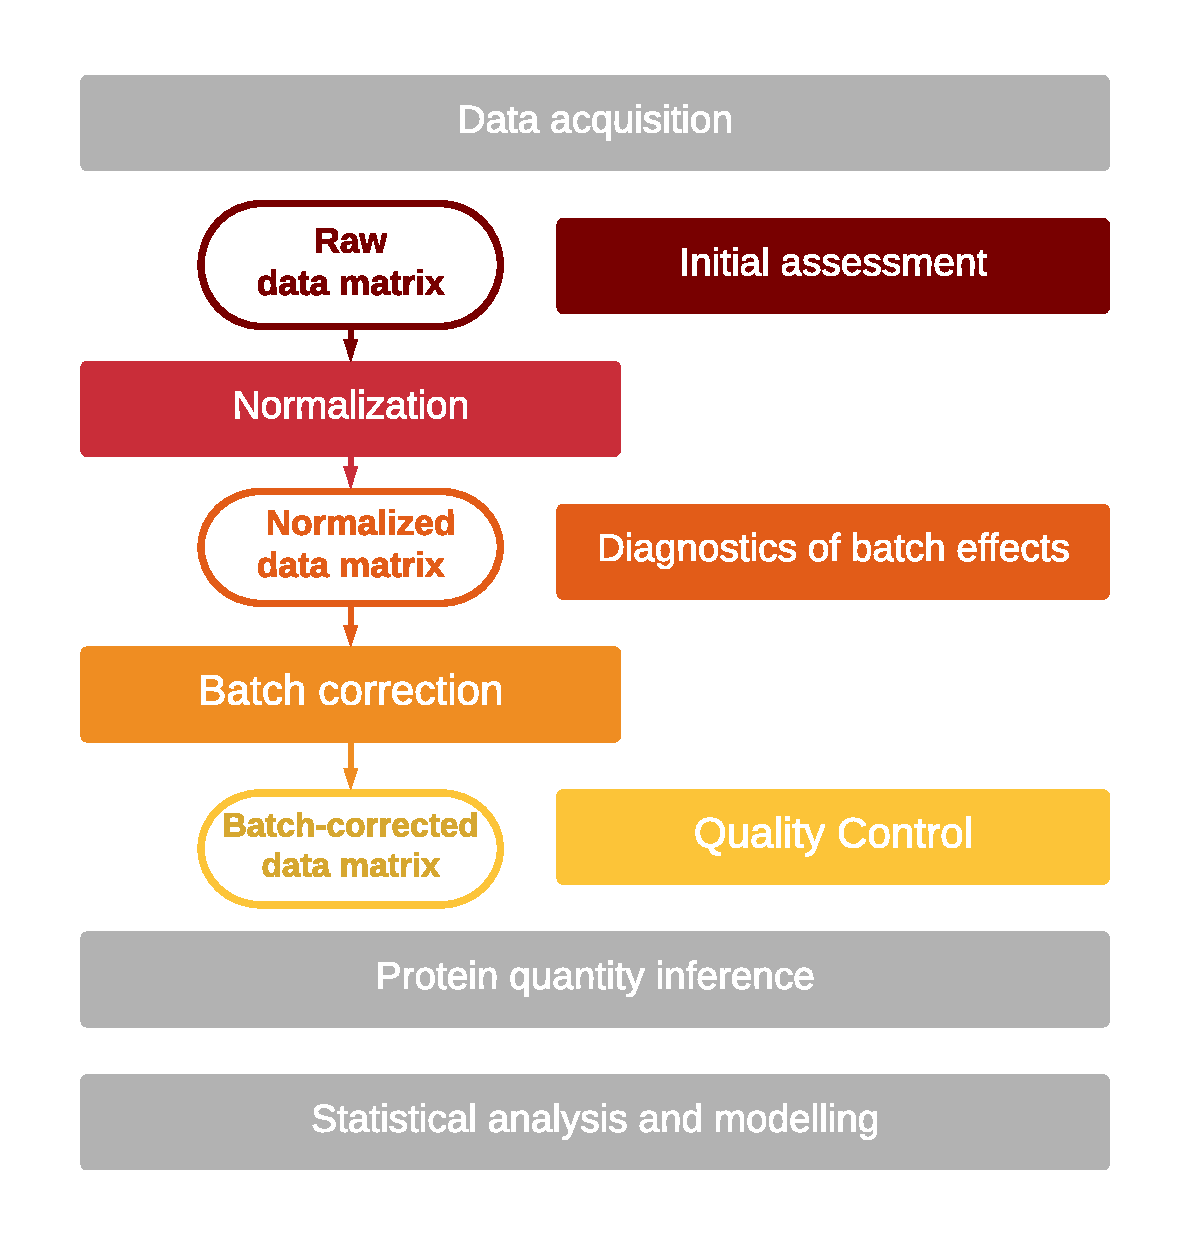
\includegraphics[width=6cm]{figures/Fig0_workflow_staircase}
	\caption[Batch effect correction workflow]
	{\textbf{Batch effect processing workflow}}
	\label{fig:batch_fig1_workflow}
\end{figure}

%We suggest a five-step workflow to address batch effects in large-scale dataset. Initial assessment allows to evaluate whether batch effects are present in raw, unnormalized data and to select normalization procedure. Second, normalization brings all samples from the dataset to the common scale, typical methods of normalization being sample-wide quantile normalization and median normalization. Third step is diagnostics of batch effects in normalized data, with methods such as PCA, hierarchical clustering. This step determines whether further correction is required. If batch effects are still present in the data, a furter step of batch correction is required. Batch correction addresses feature-specific biases, commonly addresses with tools like ComBat \cite{Johnson:2007aa} or feature-specific mean/median centering. Finally, quality control ensures that the data has been improved by correction: biases have been reduces while meaningful signal has been retained. In the next sections, we discuss each step of the workflow in more detail, illustrating it with examples from three large-scale proteomic datasets.

\subsection{Data matrix before adjustment}

This workflow starts with raw data matrix, for which initial steps, such as peptide-spectrum matching, quantification, and FDR control are completed. Data is assumed to be log-transformed, unless the variance stabilizing transformation \cite{Durbin2002} is used. In that case, data transformation gets included into the normalization procedure. 

We strongly suggest to perform the batch affect adjustment on peptide or fragment ion level, as this procedure alters feature abundances, and these abundances are critical for the protein quantity inference \cite{Clough:2012aa, Teo:2015aa}.  

Also, we encourage to keep all detected peptides, and not to filter out any measurements during batch effects adjustment. This means, that also non-proteotypic and the ones with numerous missing values should be used during batch effects adjustment procedure. Keeping all measurements allows to better evaluate the intensity distribution within each sample, which is critical for subsequent normalization and correction steps.

\subsection{Initial assessment}
In most cases, the intensities of samples are different from each other. Comparing global quantitative properties such as sample medians or standard deviations helps with the choice of normalization method and point to specific technical factors, such as MS instrument, that needs more control. 

Three approaches are useful for initial assessment: 1) plotting sample average or mean, in order of MS measurement or digestion batch, allows a precise estimation of MS drift or discrete bias in each batch; 2) Boxplots allow to assess the variance and check the samples for outliers; 3) Correlation of samples shows, whether there is a tendency of samples from the same batch to be more similar than unrelated samples. Since: samples from the same batch have no biological similarity, such correlation is a clear sign of bias.

Initial assessment sets the baseline for bias magnitude and sources and facilitates the choice of normalization method.

\begin{table}[hbt]
	\begin{tcolorbox}
		\section*{Box 2: Batch effects processing checklist}
		\label{box:Box2_checklist}
		\begin{tabular}{>{\raggedright}p{2cm}m{10.5cm}}
			\headrow
			\thead{Step} & \thead{Substeps} \\
				
			Experimental design (highlights)	& \begin{enumerate}
				
				\item Randomize samples in a balanced manner to prevent confounding of biological factors with batches (technical factors).
				\item Consider adding replicates
				\item Record all technical factors, both plannable and occurring unexpectedly 
			\end{enumerate} \\ 
			Initial assessment	& \begin{enumerate}
				
				\item Check whether the sample intensities are consistent. 
				\item Check the correlation of all sample pairs
				\item If intensities or sample correlation differ, check whether the intensities show batch-specific biases
			\end{enumerate} \\
		
			Normalization		& \begin{enumerate}
				
				\item Choose normalization procedure, appropriate for biological background and data properties;
				\item \textbf{(!)} If the goal is to determine differentially expressed proteins, and the batch effects are discrete or linear, multi-factor ANOVA on normalized data is a sound statistical approach, as it adjusts for batch effects simultaneously with identification of proteins, that are statistically significant in terms of differential expression. This is true even if diagnostic tools indicate the presence of batch effects.

			\end{enumerate} \\ 
			Diagnostics		& \begin{enumerate}
				
				\item Using diagnostic tools (See \hyperref[box:Box1_definitions]{Box 1}), determine, whether batch effects persist in the data. 
				\item Use quality control already at this step and skip the correction if it is not necessary. 
				
			\end{enumerate} \\ 
			Batch effects correction	& 	\begin{enumerate}
				\item	Choose batch effects correction procedure, appropriate for the biological background and data properties, especially those detected at the previous step
			\item	Repeat the diagnostic step
			\item	Assess the ultimate benefit with quality control
\end{enumerate} \\ 

			Quality control 	& 	\begin{enumerate}
				
				\item	Compare correlation of samples within and between the batches. Pay special attention to replicate correlation, if these are available;
				\item	Compare correlation of peptides within and between the proteins.	
			\end{enumerate} \\ 
		\end{tabular}
		
	\end{tcolorbox}
\end{table}
\clearpage

 



\subsection{Normalization}

The goal of normalization is to bring all samples to the same scale to make them comparable. Two main considerations drive the choice of normalization method: 

1) \textbf{Heterogeneity of the data: }if samples are fairly similar, the bulk of the proteome does not change and thus techniques such as quantile normalization \cite{Bolstad2003} can be used. In datasets that are dramatically different, i.e. when a large fraction of the variables are either positively or negatively affected by the treatment, different methods, such as HMM-assisted normalization can be used \cite{Landfors2011}. Additionally, if some samples are expected to have informative outliers (e.g. muscle tissue, in which a handful of proteins are several orders of magnitude more abundant then the rest of the proteome), methods that keep the relationship of outliers to the bulk proteome, need to be used \cite{Wang770115}.

2) \textbf{Distribution of sample intensities: }The initial assessment step, especially boxplots, indicate, which level of correction is required: in most cases, shifting the means or medians is enough, but when variances differ substantially, these need to be brought to the same scale as well.

It should be noted, that normalization might be the only adjustment and no further correction is required. This can be determined with the diagnostic plots and quality control methods, described below. If the results are satisfactory, keeping data manipulation minimal is always advisable.

\subsection{Diagnostics of normalized data}

Normalization makes the samples more comparable and it is possible that most of the bias is removed by it and no further processing is required. However, normalization aligns only the global patterns in the samples, while batch effects, affecting specific proteins or groups of proteins might still represent a major source of variance. Thus, diagnostic of batch effects is most informative for the normalized data. 

The diagnostic approaches can be divided in proteome-wide and peptide-level approaches. The main approaches for \textbf{proteome-wide diagnostics} are:
\begin{itemize}
	\item \textbf{Hierarchical clustering} is an algorithm that groups similar samples into a tree-like structure called dendrogram. Similar samples cluster together and the driving cause of this similarity can be visualized by coloring the leaves of the dendrogram by technical and biological factors. Hierarchical clustering is often combined with the heatmap, mapping quantitative values in the data matrix to colors, which facilitates the assessment of patterns in the dataset.
	\item \textbf{Principal Component Analysis (PCA)} is a technique that identifies the leading directions of variation, known as principal components. The projection of data on two components allows to visualize sample proximity. This technique is particularly convenient to assess clustering by biological and technical factors, or check replicate similarity (works well until about 50-100 sample in a dataset). 
	\item \textbf{Principal Variance Component Analysis (PVCA)}. PVCA maps each principal component to technical and biological factors, assessing the weight of each factor in each component. These weights are then combined with the variance fraction of each component, thus quantifying the variance, associated with each factor, both technical and biological. Thus, PVCA turns the intuition of PCA into a quantitative readout. 
\end{itemize}

One should be careful, however, in interpreting proteome-wide diagnostics, as all of them were designed for data matrices without missing values. For more details, we refer the reader to %\ref{Box_3_Missing_values}.

In proteomics \textbf{peptide-level diagnostics} are as useful as proteome-wide diagnostic. As in other high-throughput measurements, individual features, in this case peptides, are visualized to check for batch-related bias. In proteomic datasets, spike-in proteins or peptides are added as controls, and can be used for this purpose. In most DIA datasets also iRT peptides \cite{Escher:2012aa}, if added in precise concentration, are very well suited for individual feature diagnostics.
It should be noted, however, that any random peptide should not be biased in a batch-related manner, so checking a handful or regular peptides can also be informative.

Another reason to check individual peptides in proteomics is to examine the trends associated with sample running order. These trends might occur as MS signal deteriorates and such bias requires special correction approaches.

\subsection{Batch effects correction}
Diagnostics helps to determine, whether batch effects correction is needed. As global sample patterns have already been corrected on the sample level, batch effects affect specific features and feature groups, and that’s the level on which they need to be corrected.

If batch effects are continuous, i.e. manifest as MS signal drift, the order-specific curve needs to be fitted. Such drifts are more likely to occur in studies profiling hundreds of samples. Since this is a problem that is specific to mass spectrometry and is still new for the community, we propose a solutions for it in  \ref{Box_4} Box 4 “Correcting MS signal drift”.

It is more common that batch effects are discrete and manifest as feature-specific shifts of each batch. For these cases, methods such as mean and median centering work very well. A more advanced modification of the mean shift is provided by ComBat \cite{Johnson:2007aa}, that uses a Bayesian framework, which has been successfully applied to proteomic data \cite{Lee:2019aa}. However, this requires that all features are represented in each of the batches, which might filter out a prohibitively high number of peptides, especially in large-scale proteomic datasets (see \hyperref[box:Box3_missingness]{Box 3 “Missing values”} for details).

\subsection{Quality Control}

The purpose of the quality control is to determine whether the adjustment procedures – normalization and/or batch effects correction – have improved the data. At this step, the data after adjustment are compared to the raw data matrix.

There are two types of criteria to evaluate the data quality: 1) Removal of the bias (negative control); 2) Improvement of the data (positive control).

Typically, bias is considered to be removed, if diagnostic plots indicate that similarity between samples is not driven by technical factors anymore. This means that neither hierarchical clustering nor PCA show clustering by batch, and correlation of samples from the same batch is no longer stronger than correlation of unrelated samples. Also, individual features should not show batch-related biases. Thus, comparison of diagnostic plots for raw and adjusted data serves as the negative contol.

Proving the improvement is, however, much harder. It is common to take “improved clustering by biological condition” or “higher number of differentially expressed proteins” as a positive control and generally, as a sign of data quality improvement. However, both criteria can be subjective: it is impossible to know beforehand, whether biological groups are separable in the proteomic space, especially if only a subset of proteins changes and the bulk of the proteome is not. Similarly, it is not possible to predict, whether higher sensitivity for differential expression does not come at the expense of added false positive hits. This is why we do not recommend these criteria for the assessment of the method of normalization or batch effects correction: the choice of the method should rather be based on properties of the samples as described above. However, since batch adjustment removes a certain portion of variance, the coefficient of variation for peptides and proteins in replicated samples should decrease. This is especially true for spike-in peptides or protein that are added to samples in controlled quantities. 

A stronger positive control is reproducibility check. In biomedical research, one can compare lists of differentially expressed proteins or predictive performance of regression/classification models. This means, that such analysis is executed in parallel from two or more sets of samples, that originate from different batches \cite{Lazar:2013aa}. It is assumed that in adjusted datasets, the resulting lists of proteins, that are differentially expressed or optimal for class separation, will be highly overlapping \cite{Shabalin:2008aa}. If two sets of samples are independently used for predictive modeling, the predictive performance of such models is also expected to be comparable \cite{Luo2010}. This framework, however, is restricted to fairly large datasets, as predictions from small-scale experiments tend to be unstable. Otherwise, this method is particularly universal, as it is applicable to the studies, where data is acquired by different technologies (e.g. microarrays and RNA-seq for transcriptomics or DIA vs TMT for proteomics).
 
We propose two methods, that do not rely on large sample size. These positive control methods are applicable to most proteomic experiments. The first is based on correlation of samples: it is expected, that replicates correlation is higher than the correlation of unrelated samples. Although it is conceivable that occasional replicates correlate less than some unrelated sample pairs, the distribution of replicate correlations should be clearly shifted upwards and this distinction should be strengthened by batch adjustment procedures. The second assessment method is specific for bottom-up proteomics, and makes use of peptide correlation: correlation of unrelated peptides is expected to be close to zero, while peptides of the same protein are likely to be positively correlated. Since tens of thousands of peptides are routinely detected in modern high-throughput proteomic experiment this metric is a reliable readout of data quality.

\section{Dataset description (?=Materials)}\label{subsec:datasets}

To illustrate the application of the workflow described above, we use three large-scale proteomic datasets, described in the Table~\ref{tab:batch_datasets}. 

Two of these datasets are published. The first study, called here \textbf{"InterLab study"}, assessed the robustness of SWATH-MS in multi-lab setting \cite{Collins2017}. A set of 30 of stable isotope labeled standard (SIS) peptides \cite{Ebhardt2012}, partitioned in five groups, was diluted in the HEK293 cell lysate . The background of HEK293 proteome was constant, but groups of different SIS peptides were diluted serially to cover a dynamic range from a concentration range from 12 amol to 10 pmol. This created a set of five samples that were distributed to 11 participating laboratories worldwide for measurement by SWATH-MS. according to a predetermined schedule: each of the samples was run on 3 separate days, with the exception of the 4th sample that was run three times on each day. Thus technical covariates whose effect needed to be assessed were data acquisition site and day. No biological signal needed to be identified in this data. For the purpose of the workflow illustration, we examine only the effect of the acquisition site. As all changes in proteome in these data are attributed to technical covariates, all samples in this study can be treated as replicates, as only a small number of SIS peptide is different. Totally, 229 samples have been profiled. Within this manuscript, we analyzed only the influence of "site" as the batch factor.

The second study, named here \textbf{"PanCancer study"} \cite{Sajic2018}, profiled the blood proteome of the cohort of patients with five solid carcinomas and matched controls. In this project, 155 blood plasma samples were collected. Protein digestion and glycopeptide enrichment have been performed in 4 batches, several weeks apart. To ensure control of the reproducibility of the samples, 7 biospecimens were replicated and allocated to a different batch to control for measurement reproducibility. To control for intra-sample variation, bovine fetuin-B was spiked in equal amount into each plasma sample. Total of 162 samples was collected (this includes samples from the prediction cohort, but not validation cohort, in the original study).

The third dataset called here \textbf{"Aging mouse study"}, has not been published before. In this study, liver proteome of mouse from BXD reference mouse population \cite{Peirce:2004aa} have been profiled to identify proteome changes associated with age. The experimental setup, however, was similar to previous BXD mice metabolic profiling experiments \cite{Williams:2016aa}: animals of each strain were subjected to Chow and High-Fat Diet. Samples were randomized with respect to biological covariates (age, diet, sex) and two mice samples with EarTags "ET1506" and "ET1524" were injected every 10-15 samples to control for signal consistency. Samples were digested in four batches. Mass-spectra acquisition was deteriorating and this is why data acquisition was interrupted for machine cleaning and tuning six times, resulting in 7 mass-spectrometry batches, which were mostly confounded with digestion batches. To allow for evaluation of mass-spectrometry batch effect, 10 samples profiled at the end of batch 3, were profiled again after machine tuning. Totally, 375 samples were used for the analysis. \textcolor{blue}{Details about the experimental condition and proteomic profiling can be found below in section \ref{sec:mouseProteome}. \textbf{SHALL WE KEEP THIS SENTENCE and add the experimental details?}}

Thus, these datasets reflect various applications of large-scale proteomic studies: they operate with cell cultures, patient and mice samples. Importantly, these three cases represent also major types of sample-to-sample heterogeneity: while the InterLab study is very homogeneous and the samples are essentially technical replicates, the PanCancer dataset is highly heterogeneous, since as little as 295 proteins have been identified in samples originating from different hospitals and cancer localizations. Mice dataset represent an intermediate case: on one hand, these samples are genetically very similar, since mice originate from two parental mouse strains and were grown in the controlled environment. On the other hand, these are still tissue samples, that might have differences due to tissue heterogeneity.

\begin{landscape}
	\begin{table}
		\renewcommand*{\arraystretch}{1.8}
		\caption[Dataset description]{Dataset description. For aging study: number of proteins and peptides before filtering for completeness}
		\label{tab:batch_datasets}
		\small
		\begin{tabular}{|  m{1.75cm}|  m{1.15cm} |  >{\raggedright}m{1.5cm} | >{\raggedright}m{4.13cm} |  m{2.5cm} |  >{\raggedright}m{2.2cm} |  m{1.5cm} |  m{1.5cm} |}
			\hline
			\textbf{Sample} & \textbf{Organism} & \textbf{Sample source} & \textbf{Sample-to-sample heterogeneity} & \textbf{Technical factors} & \textbf{Biological factors} & \textbf{Protein (peak group) number} & \textbf{Number of samples} \\
			\hline
			\hline
			\textbf{InterLab study} & human & cell culture & very low: 
			samples come from the same tissue cultures and differ by few spike-in peptides
			& \vspace*{1em}\squishlist
			\item data acquisition sites
			\item profiling days
			\squishend
			& --- & 4077
			(31886)
			& 229  \\
			\hline
			\textbf{PanCancer study} & human & blood samples & high: 
			sample come from cancer patients and matched controls with different cancer localization
			& \squishlist
			\item protein digestion batch
			\squishend
			& \squishlist
			\item case / control
			\item cancer localization
			\squishend
			& 203 (1360)
			& 171  \\
			\hline
			\textbf{Aging mice study} & mice & liver tissue & medium: 
			samples come from population of inbred samples originating from two parental strains
			&  \vspace*{1em}\squishlist
			\item protein digestion batch
			\item MS batch
			\item MS drift
			\squishend
			& \squishlist
			\item Strain
			\item Diet
			\item Age
			\squishend
			& 5436*
			(33157*)
			& 371  \\
			\hline
		\end{tabular}
	\end{table}
\end{landscape}

\section{Case Studies}\label{subsec:case_studies}
\subsection{Initial assessment}
The main goal of the initial assessment is to set a baseline for the magnitude and nature of batch effects in a particular dataset. At this stage the data matrix is “raw” in a sense, that the quantities are reported as measured, without any calibration, normalization or correction with regard to the quantities in other samples.


\begin{figure}[hbt]
	%\center
	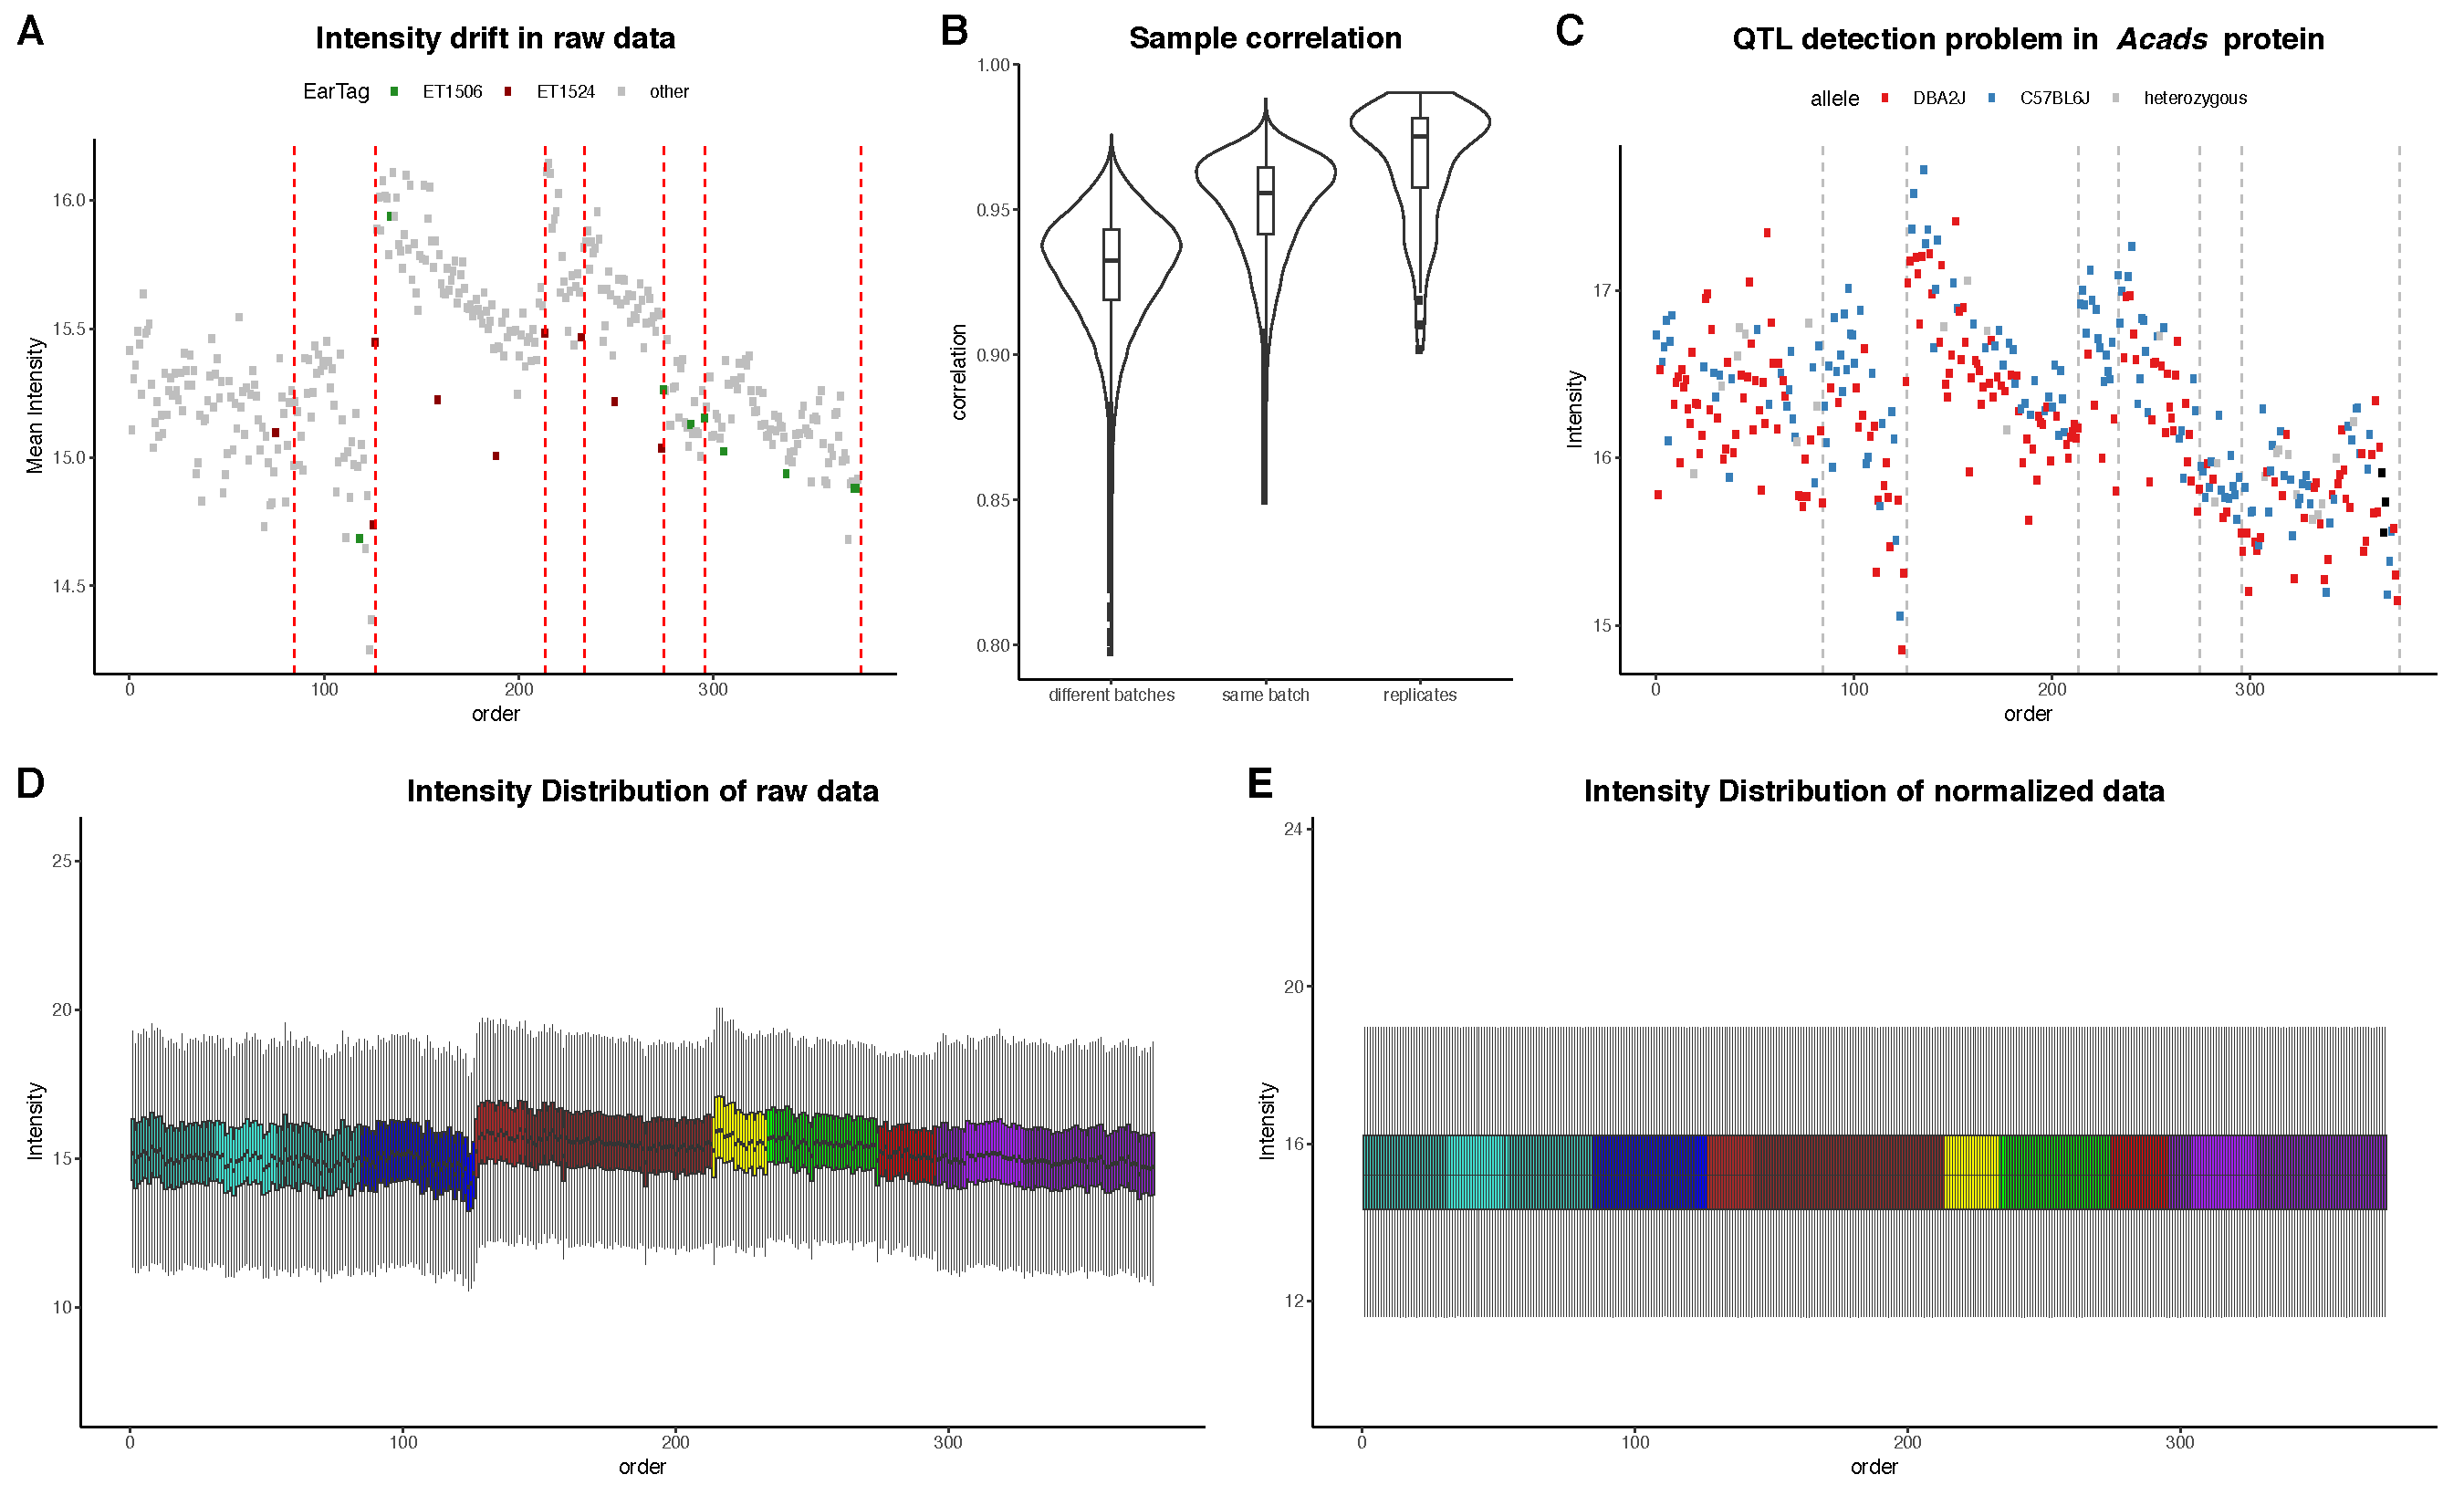
\includegraphics[width=\textwidth]{figures/Fig1_initial_assessment_v5_edited.pdf}
	
	\caption{\textbf{Initial assessment and normalization} \\
		\footnotesize
		(A) Mean Intensity in raw data vs sample running order with repeatedly replicated samples shown in color; (B) Distribution of unadjusted sample intensity correlations - between batches, within batches and in replicated samples; (C) Representative "Acads" protein QTL, that cannot be detected due to the signal drift; (D) Boxplots of sample intensities in raw, unnormalized data; (E) Boxplots of sample intensities after normalization}
	\label{fig:batch_fig2_initAssessment}
\end{figure}

Thus, it is essential to get a quick overview of the data by comparing global statistics, such as average intensity or correlation of samples, and few individual proteins, for which there is some prior information on their expected abundance. In mass-spectrometry, it is important to plot these statistics in a sample running order, as it is not uncommon, that the signal measured starts to drift. This is clearly seen on Figure~\ref{fig:batch_fig2_initAssessment}A, where average intensity is plotted vs sample running order. In this case, the intensity tended to deteriorate after 50-70 samples, and interrupting the acquisition for cleaning and calibrating the instrument determined the mass-spectrometry batch. As this type of bias is not entirely plannable, it is particularly important to randomize the samples before running and to include replicate samples for control (for more details on sample replication see Section~\ref{subsec:datasets}“Dataset description”). 

Batch effects introduce not only intensity shifts of total sample, but also lead to spurious correlation between features (in proteomics, fragments, peptides or proteins). It is common, that samples that belong to the same batch have strong correlation (as seen on Figure~\ref{fig:batch_fig2_initAssessment}B, Figure~\ref{fig:batch_figS1_InterLab}B), not only stronger than the correlation of samples from different batches (“between batches”), but often stronger than the correlation of replicates. This is why it is important to assess correlation distributions as early as possible. Sample correlation can be visualized as the square heatmap (InterLab Study, Figure~\ref{fig:batch_figS1_InterLab}B) or the correlation distribution boxplot with or without violin plot (Figure~\ref{fig:batch_fig2_initAssessment}B), first preferred with smaller sample sizes and the latter preferable for large datasets (the boundary being roughly 150 samples).

Optionally, one can complement initial assessment with the analysis of few specific individual features (peptides or proteins), for which prior information is known. In our case, we plotted several proteins with known quantitative trait loci (QTL), to see if the alleles can be separated in this dataset. However, as seen in Figure~\ref{fig:batch_fig2_initAssessment}C, in this case the intensity drift prevents QTL detection.

Finally, we would like to mention boxplot, the plot that is most powerful for initial batch effects assessment: intensity boxplots in one plot demonstrate median, quantiles and outliers. This allows to see, whether there are batch-specific intensity patterns such as shifts (as in InterLab study, see Figure~\ref{fig:batch_figS1_InterLab}A), or drifts (as in Figure~\ref{fig:batch_fig2_initAssessment}D), or no evident batch-associated pattern can be spotted (PanCancer data, Figure~\ref{fig:batch_figS2_PanCancer}A). To detect the patterns, the samples should be sorted by running order or by batch (if the batches, such as digestion batches have been randomized for running). In some cases, intensity patterns are easier to spot on average intensity plot (compare to Figure~\ref{fig:batch_fig2_initAssessment}A). Nevertheless, for most cases, boxplots allow to determine, if general intensities of samples differ substantially and whether these differences are batch-specific.

\subsection{Normalization}

The normalization is an essential step in removing bias from the data as it brings the samples to the same scale, making the measured quantities comparable. As stated in “protocol overview”, the choice of normalization should take two factors into account: 
1. heterogeneity, as assessed from previous knowledge, and 2. global quantitative sample properties, e.g. mean/median/variance, as indicated by initial assessment.

The most common type of normalization, quantile normalization \cite{Bolstad2003}, is applicable to wide range of samples and that was a method of choice for Aging mouse data and PanCancer dataset. As demonstrated in Figure~\ref{fig:batch_fig2_initAssessment}D and E (and Figure~\ref{fig:batch_figS2_PanCancer}A and B correspondingly), quantile normalization literally makes the distributions very similar: not only means or quantiles are shifted to the same range, but all quantiles, including outliers become the same. This feature that is sought after for the samples, where the majority of features are not expected to change, can become a problem in cases, where outliers bear important information.

Median centering normalization only brings the medians to the same scale and thus is a “mild” normalization. This is the type of normalization that has been applied to InterLab study. This normalization improved the made the quantities of peptides as measured at different sites much closer than they were before (see Figure~\ref{fig:batch_figS1_InterLab}C). Thus, shifting the medians to the same value (see Figure~\ref{fig:batch_figS1_InterLab}D) removed substantial portion of bias and thus achieved the goal of making the measurements in different samples comparable. The improvement of the signal quantity is also seen from the improved protein quantification precision: coefficient of variation has shrunk for the majority of proteins (see Figure~\ref{fig:batch_figS1_InterLab}E).

This means, that in certain cases normalization alone is sufficient and no further correction is needed. In this case, improvement of quantification of spike-in peptides (Figure~\ref{fig:batch_figS1_InterLab}C) and the decrease in protein coefficient of variation (Figure~\ref{fig:batch_figS1_InterLab}E) serves as quality control, skipping the intermediate batch correction step.

In other cases, however, additional correction of batch effects is needed to complete the adjustment of the data. Whether the correction of batch effects is needed, can be determine with batch effects diagnostics.


\subsection{Diagnostics}

\begin{figure}[hbt]
	%\center
	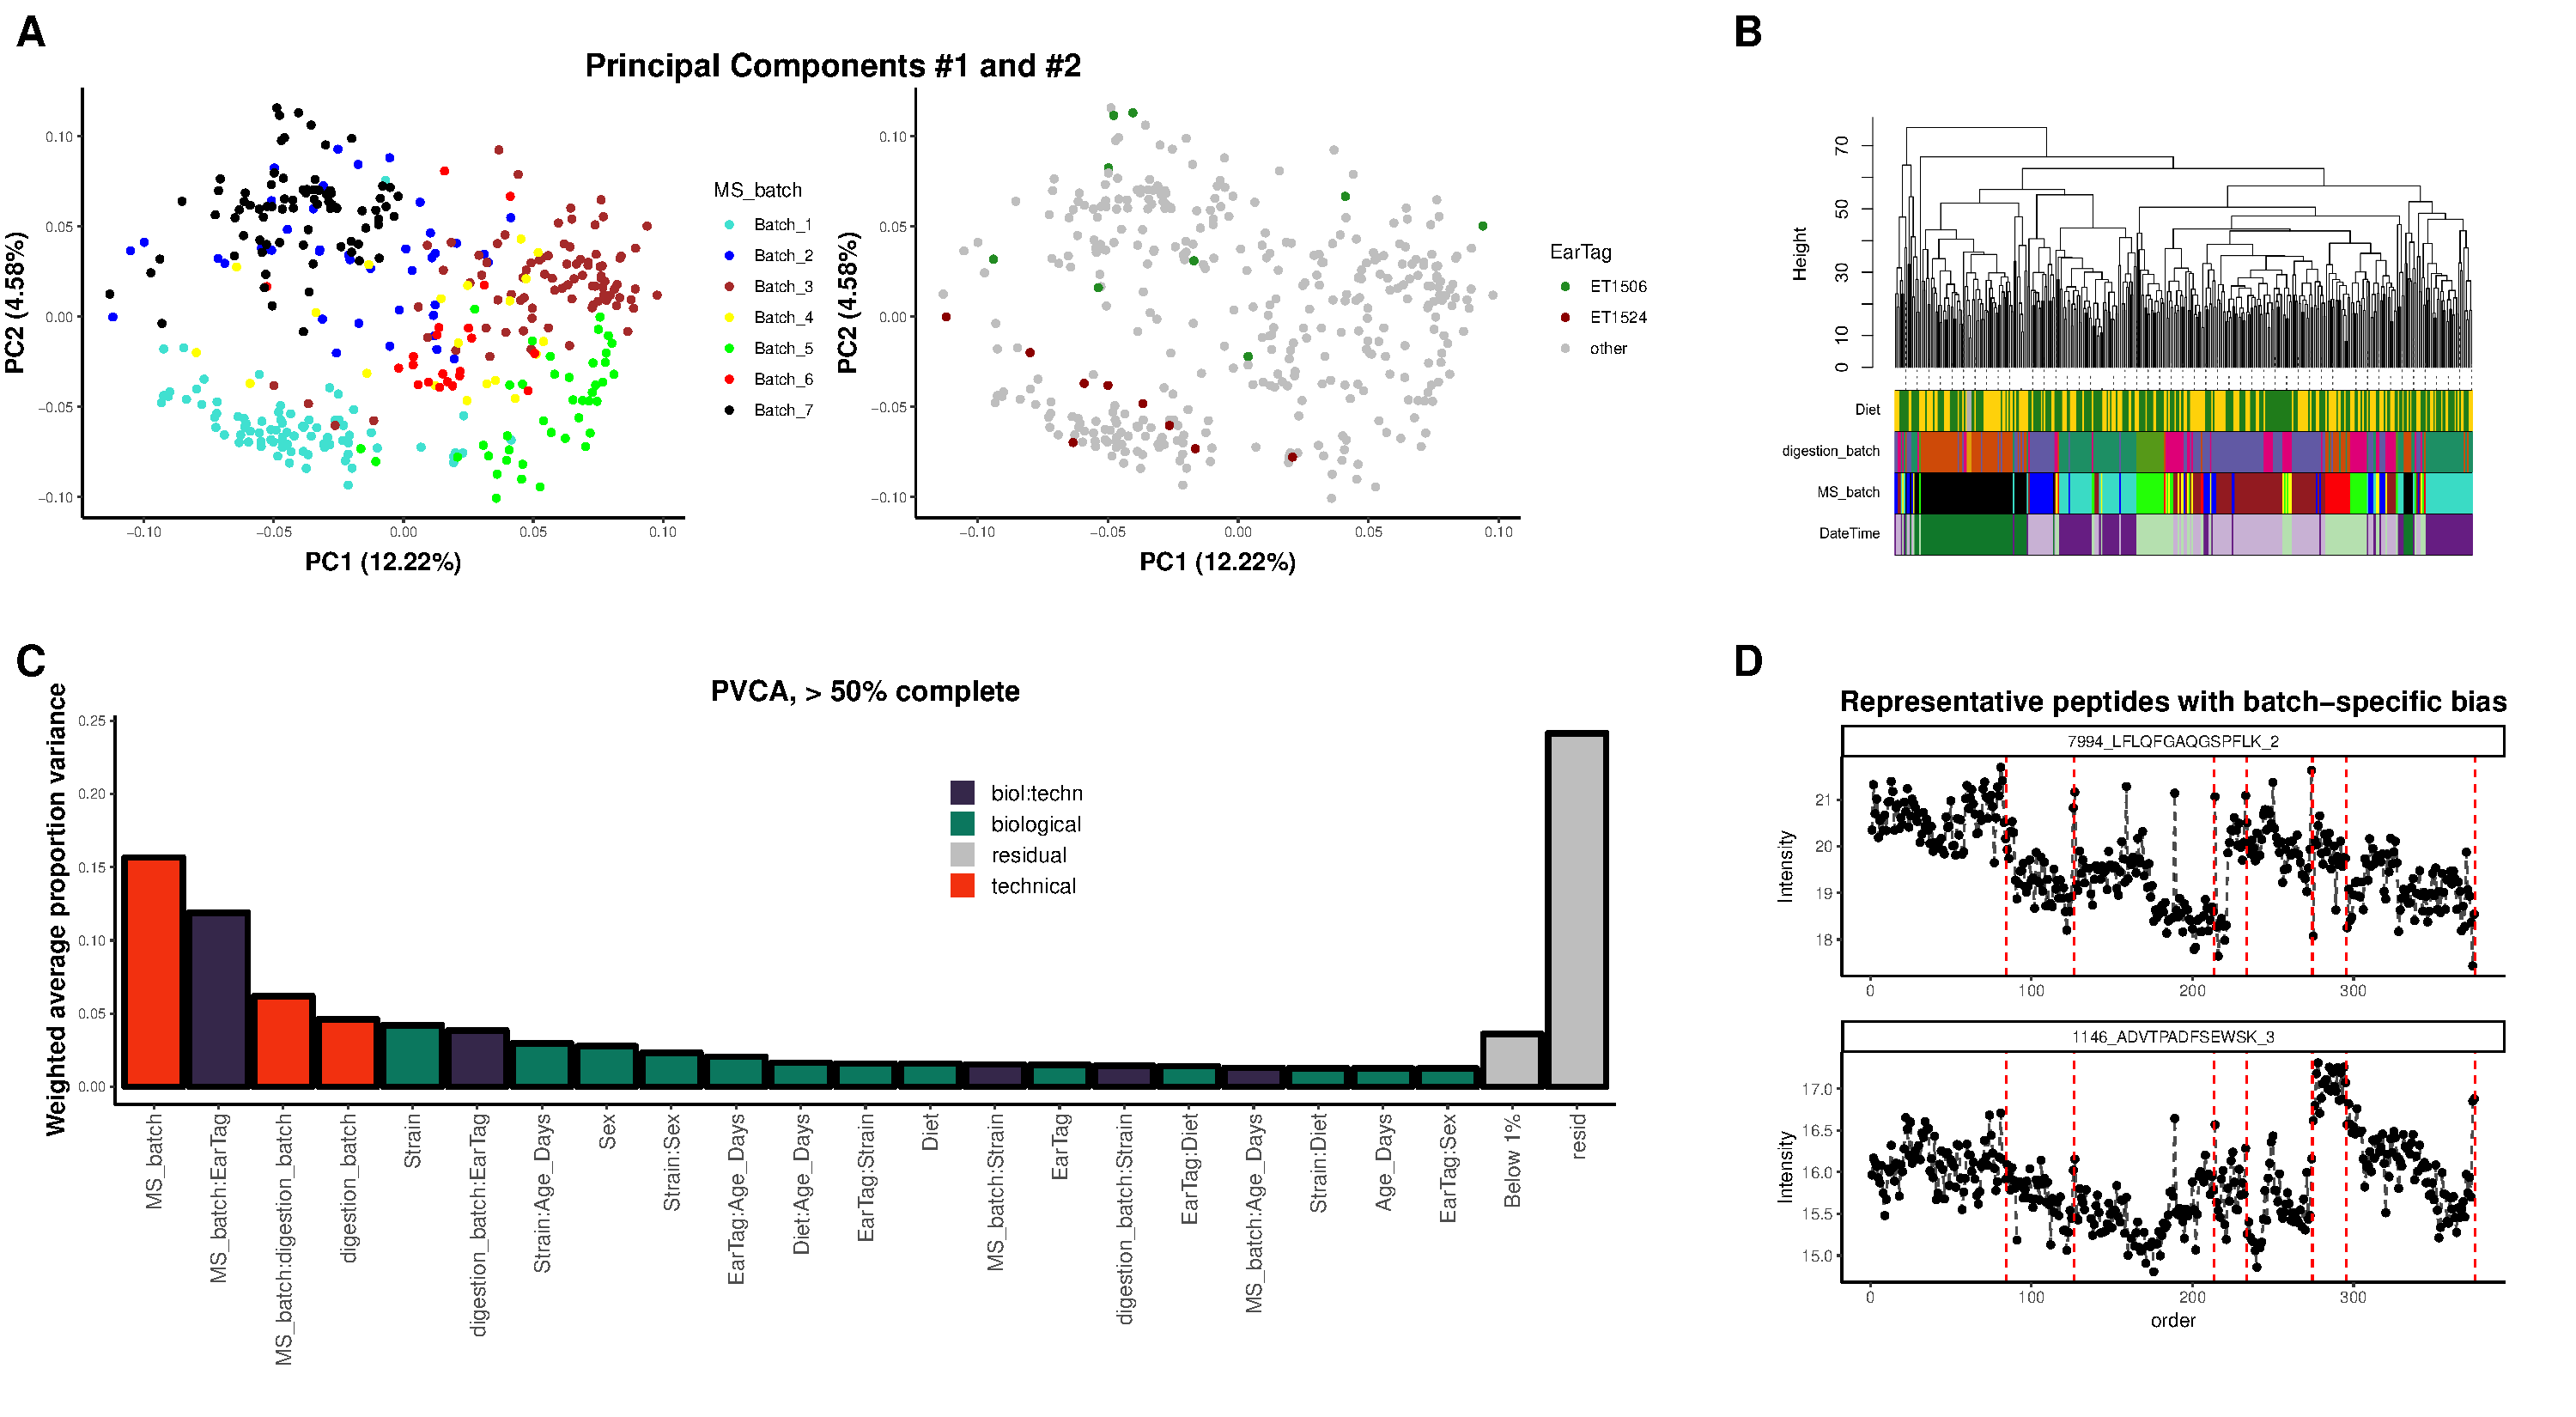
\includegraphics[width=\textwidth]{figures/Fig2_diagnostics.pdf}
	
	\caption{\textbf{Diagnostics of batch effects}  \\
		\footnotesize
		(A) Principal Components \#1 and \#2 colored by MS batch (left) and Replicates (right), where the effect of clustering by batch is dominating, but the replicated samples are closer to each other than just random samples; (B) Hierarchical clustering of samples, with leaves colored by Diet, digestion batch, MS batch and Date-time of sample acquisition: domination of technical factors is clearly visible; (C) Principal Variance Component Analysis of peptides, detected in >50\% of samples demonstrates, that the technical factors, such as MS batch, digestion batch and their combination has profound effect on the data, while biological factors such as Strain, Sex and Age account for much smaller fraction of variance; (D) Peptide-level plots for two iRT peptides demonstrate, that batch effect manifests also as MS signal drift that requires correction}
	\label{fig:batch_fig3_diagnostics}
\end{figure}

Normalization harmonizes overall sample intensities, however, batch effects can still be present and bias the quantities of many peptides and proteins.
Various methods can be used to assess the extent of bias in the data. Most of them characterize the dataset as a whole, thus working on proteome level. Methods like Principal Components Analysis and Hierarchical Clustering are the most established as they allow to visualize factors, underlying the similarity of the samples.
Principal Component Analysis (PCA) is a method that transforms the data matrix into a linear combination of “components” representing directions of highest variance in the data. This is why plotting first few components and coloring the samples by technical and biological factors or highlighting replicated samples provides a way to check, what drives the sample proximity. In Aging Mice, this makes certain patterns apparent (see Figure~\ref{fig:batch_fig3_diagnostics}A): first, we see a strong clustering of samples by mass spectrometry batch; second, replicates tend to be close, although they are not necessarily the samples with the smallest distance to each other. Each factor, however, needs a separate plot, and the figures, illustrating the influence of such factors as digestion batch, diet or acquisition date can be found in \textcolor{red}{Supplementary Fig3A}.
 
Hierarchical clustering in contrast, allows to visualize multiple factors at once (Figure~\ref{fig:batch_fig3_diagnostics}B). In principle, it shows information, similar to that of PCA: batch factors, primarily MS batch and digestion batch cluster together, while the effect of diet, the biological factor, is not as strong. Similarly, in PanCancer study (Figure \ref{fig:batch_figS2_PanCancer}\textcolor{red}{E and F\textbf{TODO: swap with hierarchical}}), we see that the digestion batch is the key factor, determining, which samples cluster together.

Principal Variance Components Analysis (PVCA) transforms the intuition of visualization brought about by PCA and Hierarchical Clustering into numbers: the weights of each factor in each Principal Component are combined, thus providing a concise summary of variance distribution between biological and technical factors and their combination. Thus, for Aging Mice dataset we see in Figure~\ref{fig:batch_fig3_diagnostics}C, that technical factors such as MS batch, digestion batch and their combination are leading drivers of variance, while biological factors, such as Diet, Sex and Age are much less prominent in the data. It should be noted, that substantial fraction of variance is “residual”, or cannot be explained by annotated sample characteristics.

One should note, however, that most proteome-wide diagnostics rely on data matrices without missing values, so typically for PCA or hierarchal clustering the missing values are filled with zeros, small random numbers etc. Since missing values are often batch-specific, this might lead to overestimate of the batch-related clustering. For more details on the effect of missing values, please refer to \hyperref[box:Box3_missingness]{Box 3 “Missing values”}.

In addition to proteome-wide diagnostics, it is highly advisable to a few individual features to control for the feature-level bias. Spike-in peptides and proteins are particularly handy for this type of diagnostics. In Aging Mice data we picked iRT peptides, that were spiked in the same quantities. In Figure~\ref{fig:batch_fig3_diagnostics}D, one can see, that despite the correction batch-specific bias affects the signal. Moreover, this bias is order-related and manifests differently for each of the peptides (for example, in samples \textcolor{red}{125 – 206}). In PanCancer, other type of peptides is used for control: there, we see that the peptides of spiked-in Bovine proteins Fetuin B and Albumin, are quantified differently in each batch (Figure \ref{fig:batch_figS2_PanCancer} \textcolor{red}{C and D \textbf{TODO: swap with hierarchical}}). There is no order-related drift, but each batch mean is clearly shifted. Thus, feature-level bias can be very different in each dataset, but checking several representative peptides is valuable to understand the nature of bias in each case.

Together, proteome-level and feature-level diagnostics guide the choice of batch correction procedure.

\afterpage{%
	\begin{tcolorbox}
		\section*{Box 3: Missing values}
		\label{box:Box3_missingness}
		Proteomics experiment now routinely profiles hundreds or thousands of proteins, however, detecting all proteins without missing values across hundreds of samples is not yet feasible. The patterns of "missingness" are known to be batch-specific \cite{Karpievitch2012}, which is also true for Aging Mice data (see Figure~\ref{fig:batch_fig4_missing_values} \textcolor{red}{\textbf{\hl{and Supp Fig X}}} for details).
		
		It should be noted, that although "missingness" among low-abundant proteins and peptides is more common, this problem can arise due to interference of peptides regardless of their abundance. 
Missing values affect the batch effects correction: methods such as ComBat \cite{Johnson:2007aa} in their current implementation don't work if the peptide is missing in at least one batch. One solution is to filter out peptides with missing values before the batch correction \cite{Lee:2019aa}, although this potentially leads to the loss of valuable quantitative data. Thus, methods such as median-centering, being more robust to the missing value problem, might be better suited for proteomic data.
		
		Missing values are often imputed, by filling with zeros, random small values \cite{Tyanova:2016aa} or re-quantification of elution traces \cite{Rost2016}. Such imputation, however, can introduce bias that is batch-specific or peptide-specific, as seen in  \textcolor{red}{\textbf{\hl{(Supp Fig Xa)}}}. This bias skews the diagnostics, such as hierarchical clustering, PCA or PVCA: batch effects will be overestimated, as clustering pattern will be driven by missing values Fig~\ref{fig:batch_fig4_missing_values}A. One way to circumvent this effect is to vary the fraction of missing values to assess, to what extent the batch effects are driven by shifts in consistently quantified peptides vs technical missingness patterns \textcolor{red}{\textbf{\hl{Supp Fig Xb}}}.
		
		Imputed values may bias the downstream conclusions As shown in Fig ~\ref{fig:batch_fig4_missing_values}B and C, if "requant" values are used, the correlation within batches seems higher than the correlation of replicates, indicating poor data quality, while with "no requants" the replicates correlate higher than other samples. 
		
		For many downstream analysis techniques, such as differential expression or protein correlation analyses, missing values are not a problem, provided that there are enough confidently quantified values. Thus, we advise to avoid imputation, or perform it after batch correction. 
		
		\begin{minipage}[h]{\linewidth}
			%\center
			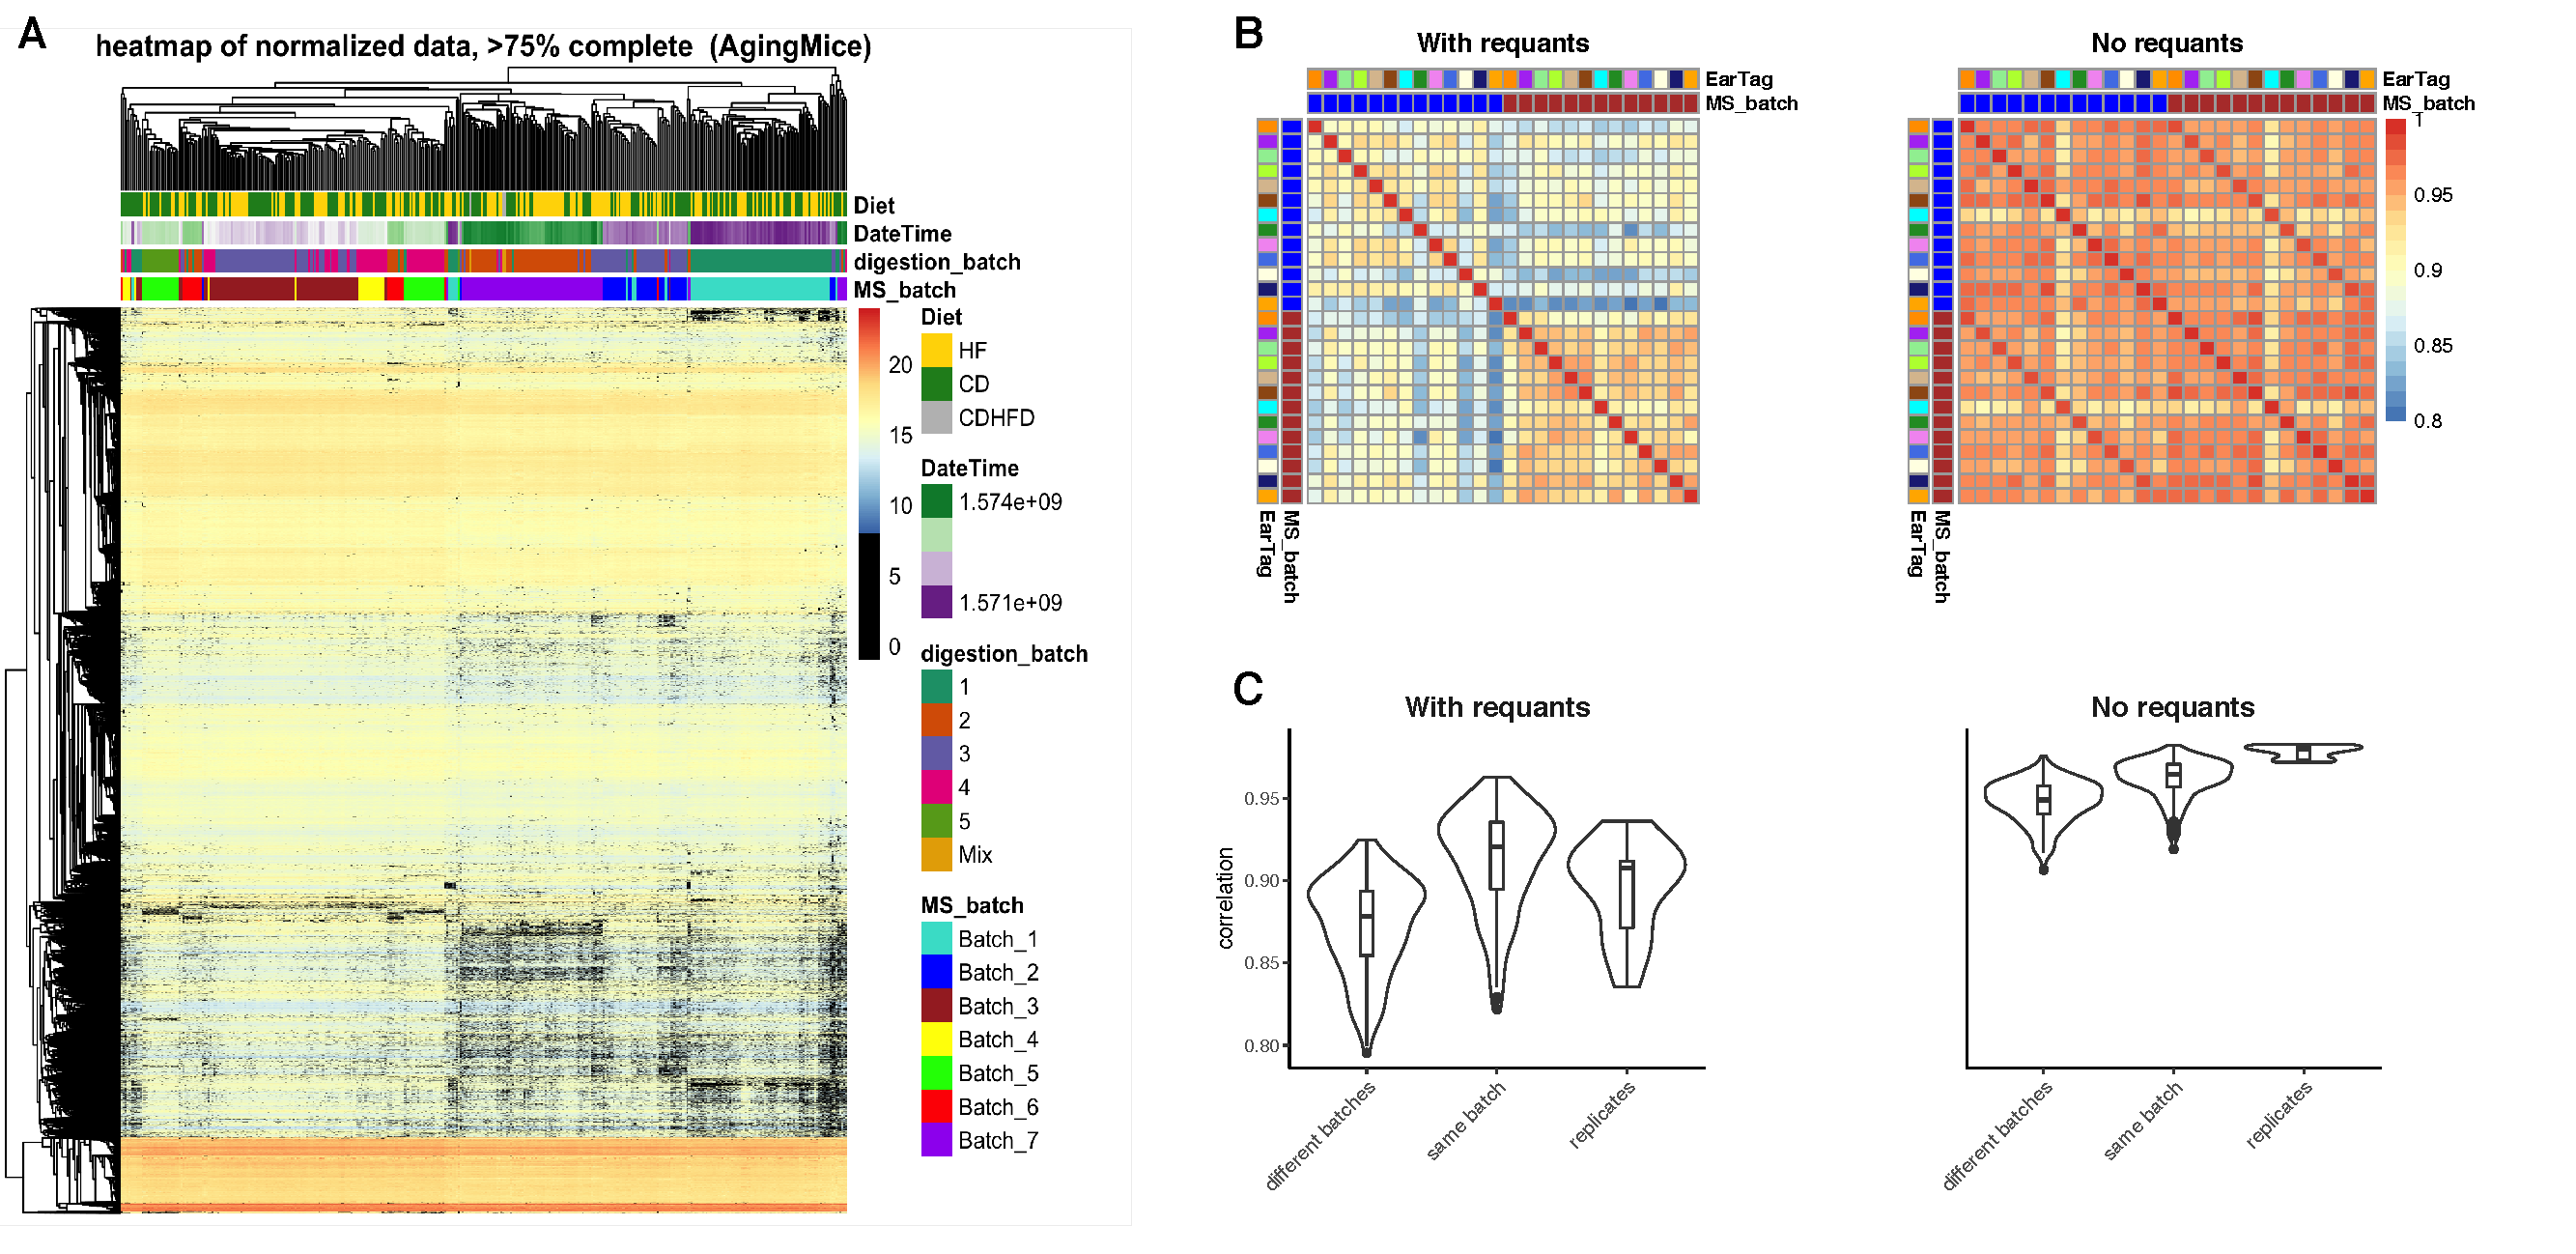
\includegraphics[width=.9\textwidth]{figures/Fig4_missing_values.pdf}
			\captionof{figure}[l]{\textbf{The problem of missing values in batch effect diagnosis and correction} }
			\label{fig:batch_fig4_missing_values}
			{\footnotesize  (A) Hierarchical clustering of normalized data; Missing values are shown in black. The missing values are non-randomly associated with the batch;
				(B) Heatmap of selected sample correlation: stronger correlation of samples within Batch 2(blue) and Batch 3 (brown) is visible in the data with "requants", and replicate correlation is much more prominent in the data without "requants";
				(C) Distribution of selected sample correlation: same effect, as in (B) is shown with violin plots of sample correlation.}
		\end{minipage}
	\end{tcolorbox}
	\clearpage
}


\subsection{Batch effects correction}
\begin{figure}[hbt]
	%\center
	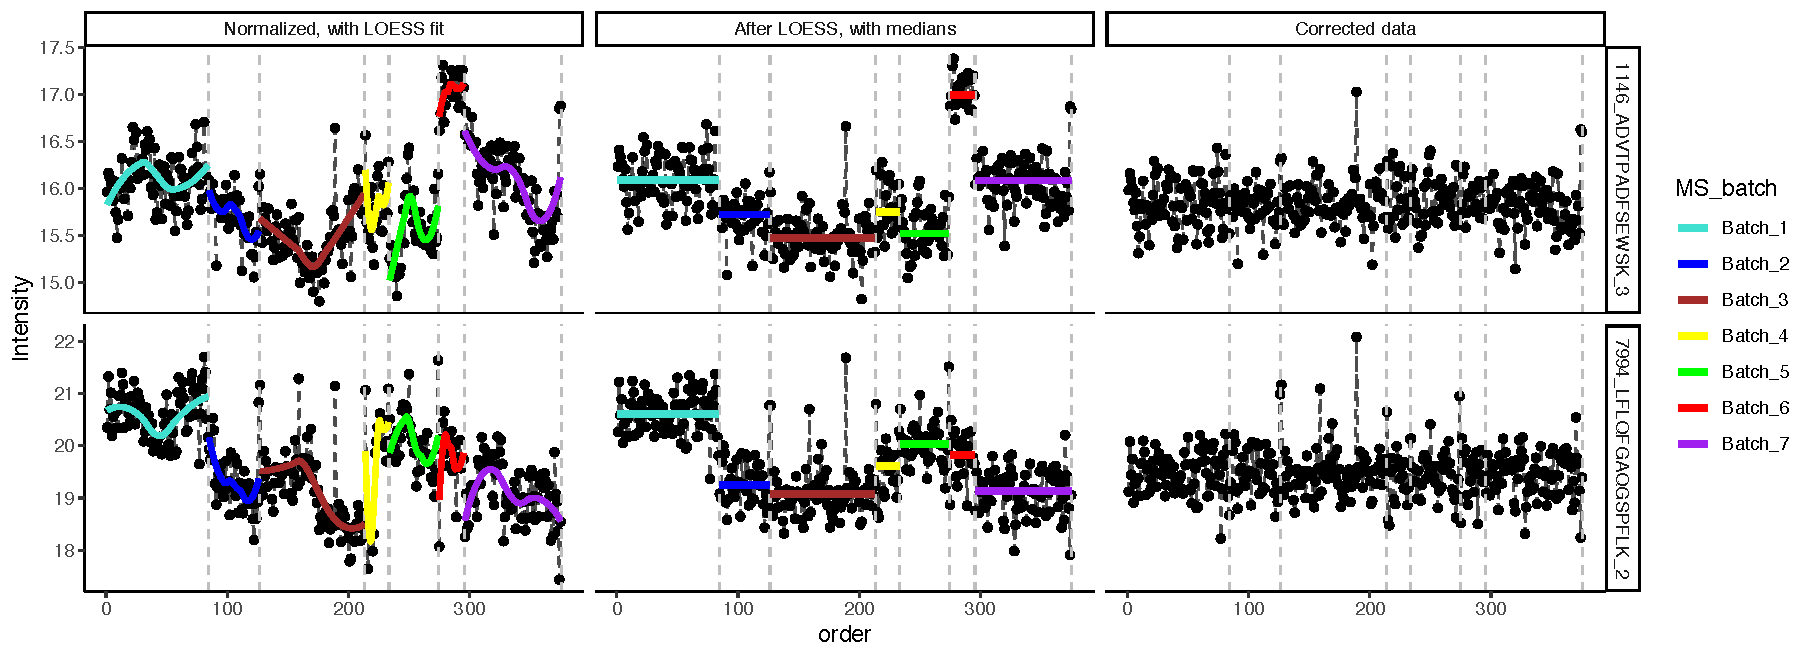
\includegraphics[width=\textwidth]{figures/Fig5_batch_correction.pdf}
	
	\caption{\textbf{Two-step correction of batch effects}  \\
		\footnotesize
		(A) Fitting LOESS curve for every peptide in each batch and subtracting the fit; (B) Using medians for correction of the residual discrete batch effect; (C) The corrected data does is more uniform and can now be used for downstream analysis}
	\label{fig:batch_fig5_batchCorrection}
\end{figure}
The goal of batch effects correction is to alleviate the bias, that remained after normalization. In most cases, normalization significantly reduces the unwanted variance (see representative peptides in \textcolor{red}{Supplementary Fig. 3C}), and, as in InterLab study, the normalization alone might be the only adjustment step. However, in many cases, different features manifest batch effects differently, as seen in Figure~\ref{fig:batch_fig3_diagnostics}D and Figure~\ref{fig:batch_figS2_PanCancer}E. Thus, batch effects correction typically is a feature-level correction.

Feature-level bias in proteomics can be of various nature: in Aging Mice data, the peptides have order-specific, continuous, bias, while PanCancer data has more common discrete shift, that can be corrected with methods, established by genomics community. 

The signal drift, as seen in Aging Mouse data, is characteristic of particularly large datasets: current generation of mass-spectrometers can typically measure consistently around 70-100 samples, but the cases when the machine can run non-stop for 150 or more samples are rare. Thus, Aging Mice, comprised of almost 400 samples, had to be split into 7 mass-spectrometry batches, with unique signal drifting pattern within it.

To address this complex bias that includes, signal drift problem, we have developed a two-step batch correction procedure shown in Figure~\ref{}.
The first step, correcting MS signal drift is based on non-linear curve fitting. As a curve-fitting algorithm, we have chosen LOESS, as it combines computational simplicity with relative flexibility of the fit characteristics. In principle the procedure runs as follows: for each peptide and each batch, a unique curve is fitted (Fig.4A), then subtracted from the normalized intensity value in each sample, leading to measurements, whose median is different in each batch (Fig 4B). At this stage the batch effects can be treated as discrete and thus discrete batch effects correction procedure can be applied. Discrete batch effects are a known problem in genomics field and thus the methods, such as median centering, ComBat and others can in principle be applied from this step on. One of the main limitation of porting the methods could be a substantial fraction of missing values, for more details on missing value problem see \hyperref[box:Box3_missingness]{Box 3 "Missing values"}.

To correct for discrete effects, in Aging Mice data we choose median centering, as most of the bias at this point can be corrected by a simple shift of the median, leading to much smoother measurements (Fig. 4C). The same procedure has been applied to PanCancer study. 

When several batch factors affect the data (as diagnosed by PCA, Hierarchical clustering and/or PVCA), all factors should be accounted for during correction. This typically means that batch factors get combined. In Aging Mice study, there were also two factors: MS batch and digestion batch. These factors, however, were highly confounded, and, when combined, certain batches would only be composed of \textcolor{red}{(X, Y, Z)} samples. Thus, it was decided to correct for MS batch only.
Thus, batch effect correction removes variance from known, annotated, batch factors. Whether the adjustment procedures – normalization and batch effects correction – improve the data signal, has to be determined by quality control.


\subsection{Quality Control}
\begin{figure}[hbt]
	%\center
	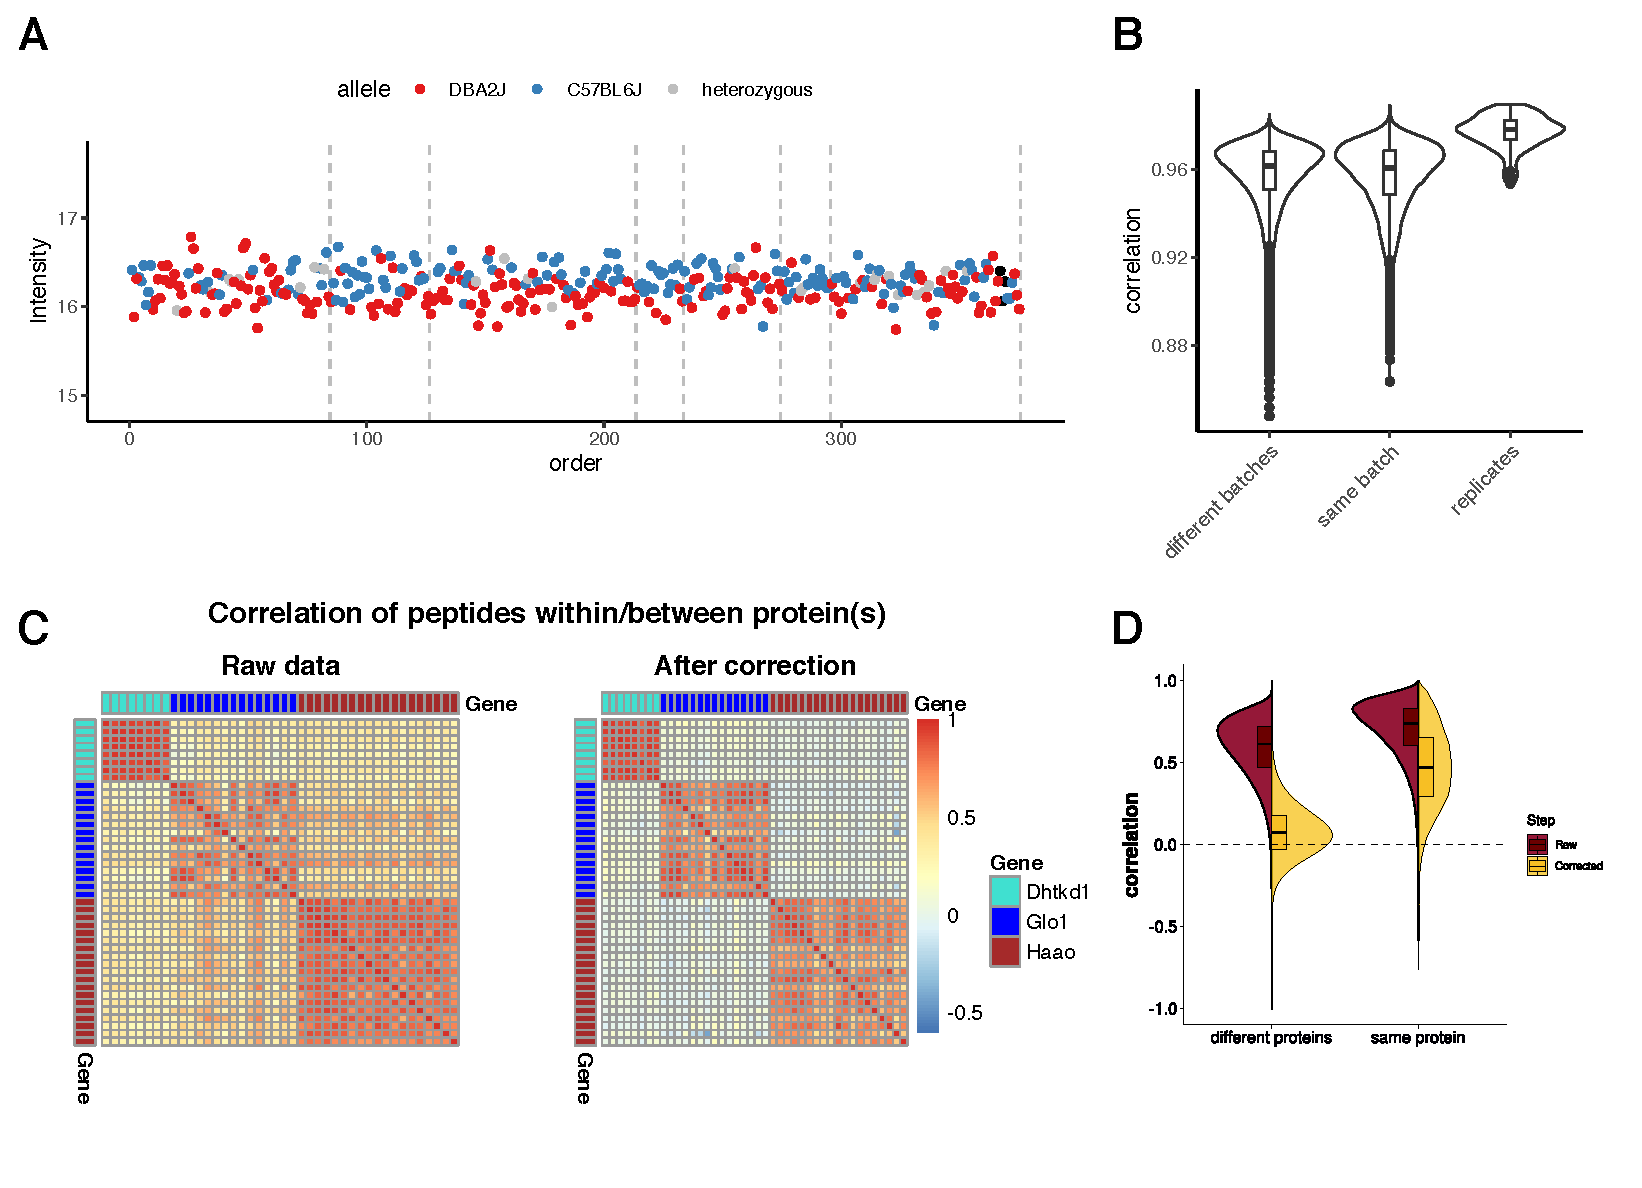
\includegraphics[width=\textwidth]{figures/Fig5_quality_control2.pdf}
	
	\caption{\textbf{Quality control of batch effects correction}  \\
		\footnotesize
		(A) Representative "Acads" protein QTL, that in corrected data demonstrates a clear allele separation; (B) Distribution of sample correlations - between batches, within batches and in replicated samples for corrected data; (C)  Heatmaps of peptide correlation for the proteins DHTKD1, GLO1 and HAAO, before and after correction: correlation is positive for all peptides in raw data, while after batch correction the correlation of unrelated peptides becomes close to zero; (D) Distribution of peptide correlation in raw data (brown) and in batch corrected data (yellow) for peptides from different proteins and peptides from the same protein: while same-protein peptide correlation is always higher than the correlation of unrelated peptides, the correlation of unrelated peptides approaches zero only after the correction.}
	\label{fig:batch_fig6_QualityControl}
\end{figure}

The main goal of the quality control is to determine, whether the data quality has improved. There are two types of quality control. Negative control, signify that biases, detected at initial assessment or diagnostic steps are not affecting the data. Positive control indicates that the data quality has improved. Certain quality control are a mixture of both types.

Negative control examples are diagnostic plots like individual peptides, PCA, hierarchical clustering or PVCA. In most cases, these show that samples are not affected by batch-specific patterns anymore (See examples for PanCancer study of corrected Bovine peptides - Figure~\ref{fig:batch_figS2_PanCancer}E and F -  and hierarchical clustering  in Figure~\ref{fig:batch_figS2_PanCancer}C and D \textcolor{red}{TODO: swap the figure this way!}). Since batch factors were specifically adjusted for at the previous step, this is in a sense a self-fulfilling prophecy. \textcolor{red}{Maybe add hierarchical clustering of Mice before and after?}

It is also common to judge the improvement by better biological signal.  In Aging Mice study, one way to measure biological signal strength is to assess the number of Quantitatative Trait Loci (QTL), particularly cis-QTLs, which means that the allele of a specific gene is affecting the expression on protein level. As seen on Figure~\ref{fig:batch_fig6_QualityControl}A, certain proteins become clearly easier to separate and less biased than before the bias adjustment (compare to Figure~\ref{fig:batch_fig2_initAssessment}C). This means, that although these cases are strong QTLs visible to the naked eye, they cannot be detected statistically due to technical bias. After normalization, the situation is very much alleviated: in addition to \textcolor{red}{XYZ} QTLs detectable in raw data, additional \textcolor{red}{ABC} alleles pass the significance threshold. Batch effects correction adds another \textcolor{red}{DEF} alleles. This essentially indicates that most of the batch effects are adjusted for at the normalization step, supporting the choice of normalization to be the only batch adjustment step.

In most cases, however, biological signal improvement is judged by “better”clustering by biological group, clustering by disease/normal, as see on PCA or Hierarchical clustering, or higher weight of that biological factor in PVCA. This approach is dangerous for two reasons. First, it is “self-fulfilling prophecy” effect: when other variance factors are removed, weight can get redistributed to other factors. Second, the grouping by biological factor (such as diseased/normal) is only a hypothesis and true differences might be small and affect only a handful of genes and proteins, and not be seen so much on the clustering. Thus, it’s not appropriate to state “the correction did not work” if clustering has not improved, and, even more importantly, this approach cannot be used as a criterion to choose a normalization or correction procedure, without justifying it by other criteria as the heterogeneity of samples or differing sample/feature variances within each batch.
Thus, clustering or PVCA, are good and valuable as negative control, but cannot be the only methods to control for the improvement of the data. We propose two approaches, that can be used in almost any proteomic experiment.

First method is based on sample proximity assessment (proximity is commonly measured as correlation). Two comparisons are important here: 1. correlation of samples from the same batch vs correlation of unrelated samples; 2. Correlation of replicates vs all other correlations. Unbiased data should not have higher correlation of same-batch samples, and replicates should clearly be more similar than a pair of unrelated samples. Instead of comparing selected sample pairs, we advise to compare the distributions of correlation coefficients. Then, it becomes clear, that although there might be cases, when two replicates have lower correlation than two unrelated samples, as a distribution, replicate correlation is clearly stronger (see Figure~\ref{fig:batch_fig6_QualityControl}B) and more prominent than before adjustment (compare to Figure~\ref{fig:batch_fig2_initAssessment}B). Most notably, however, that now the correlation distribution for the same-batch or unrelated samples is essentially identical, while the correlation of the same-batch samples was clearly stronger before the adjustment for Aging Mice dataset. Correlation, however, is not the only method to analyze sample proximity. The proximity can be analyzed with hierarchical clustering, and distance measures like \textcolor{red}{check the distance for this data - Mahalanobis?}. For example, in PanCancer dataset we see in Figure~\ref{fig:batch_figS2_PanCancer}, that the replicates were scattered in the dendrogram, while after correction, most of them cluster together. Tree-based visualization, however, becomes tricky with too many samples, with the limit of roughly ~150 to be distinguishable by naked eye. Proximity-based quality control is applicable to any “omic” dataset that has replicated samples and batches, can be tested, making this method very universal. 

Second method is specific for proteomics. Here, we utilize the fact that essentially, we are measuring the peptides or even fragments, but not the proteins themselves. This means that we can compare the correlation of peptides that are attributable to the same protein to correlation of peptides that belong to unrelated proteins. Thus, we see, that although even in the raw data peptides of the same protein correlate stronger, the peptides pairs from unrelated proteins also correlate. This effect is true not only to selected proteins (Figure~\ref{fig:batch_fig6_QualityControl}C left) but holds for the whole proteome (Figure~\ref{fig:batch_fig6_QualityControl}D, dark brown). The correlation of unrelated peptides, however, gets much closer to zero after the correction (Figure~\ref{fig:batch_fig6_QualityControl}C right, and Figure~\ref{fig:batch_fig6_QualityControl}D yellow). This means, that before correction most of the peptide correlation was spurious, and that might affect the precision of protein quantification for methods, that rely on peptide correlation.

Thus, both sample proximity and peptide correlation are powerful positive controls as they are able to indicate the improvement of the data for any biological experiment type.

With the quality control methods described, both positive and negative, it is possible to understand whether the quality of the data improved. It is, however, important, that experimental design with no confounding of technical and biological factors and with replicated samples is critical for the data to be adjustable and the correction to be controllable. It is also essential to remember, that quality control methods are not criteria to choose the method of adjustment, but their purpose is to provide metrics to control the quality of the data before and after adjustment.







\section*{Supplementary files}
Links to the data files, proBatch code, manuscript code.

\section*{Contributions}

Contributions
J.~Č and P.~P. designed the analysis workflow and wrote the manuscript, E.~W. introduced multiple components in the workflow and made major contributions to the manuscript outline and text. J.~Č., C. ~L., E.~W. and V.~S. performed data analysis. J.~Č., C.~L. and P.~P. implemented back-end R functionality, E.~W. helped with the code testing. E.~W., T.~S. and B.~C. provided proteomic data and contributed to workflow conceptualization. M.~R.-M. provided critical input on the project and assisted in analysis pipeline design. P.~P. and R.~A. supervised the study.

\section*{Acknowledgements}
1. Guy who wrote "split violinplot" function. Qing Zhong and Rebecca Poulos for early feedback on the pipeline and all Aebersold lab for critical comments and questions.

\section*{Conflict of interest}
Authors declare no conflict of interests


\printendnotes

% Submissions are not required to reflect the precise reference formatting of the journal (use of italics, bold etc.), however it is important that all key elements of each reference are included.
\bibliography{batch_references}

\graphicalabstract{example-image}{Please check the journal's author guidelines for whether a graphical abstract, key points, new findings, or other items are required for display in the Table of Contents.}

\newpage
\section{Supplementary Material}
\beginsupplement

\begin{figure}
	\centering
	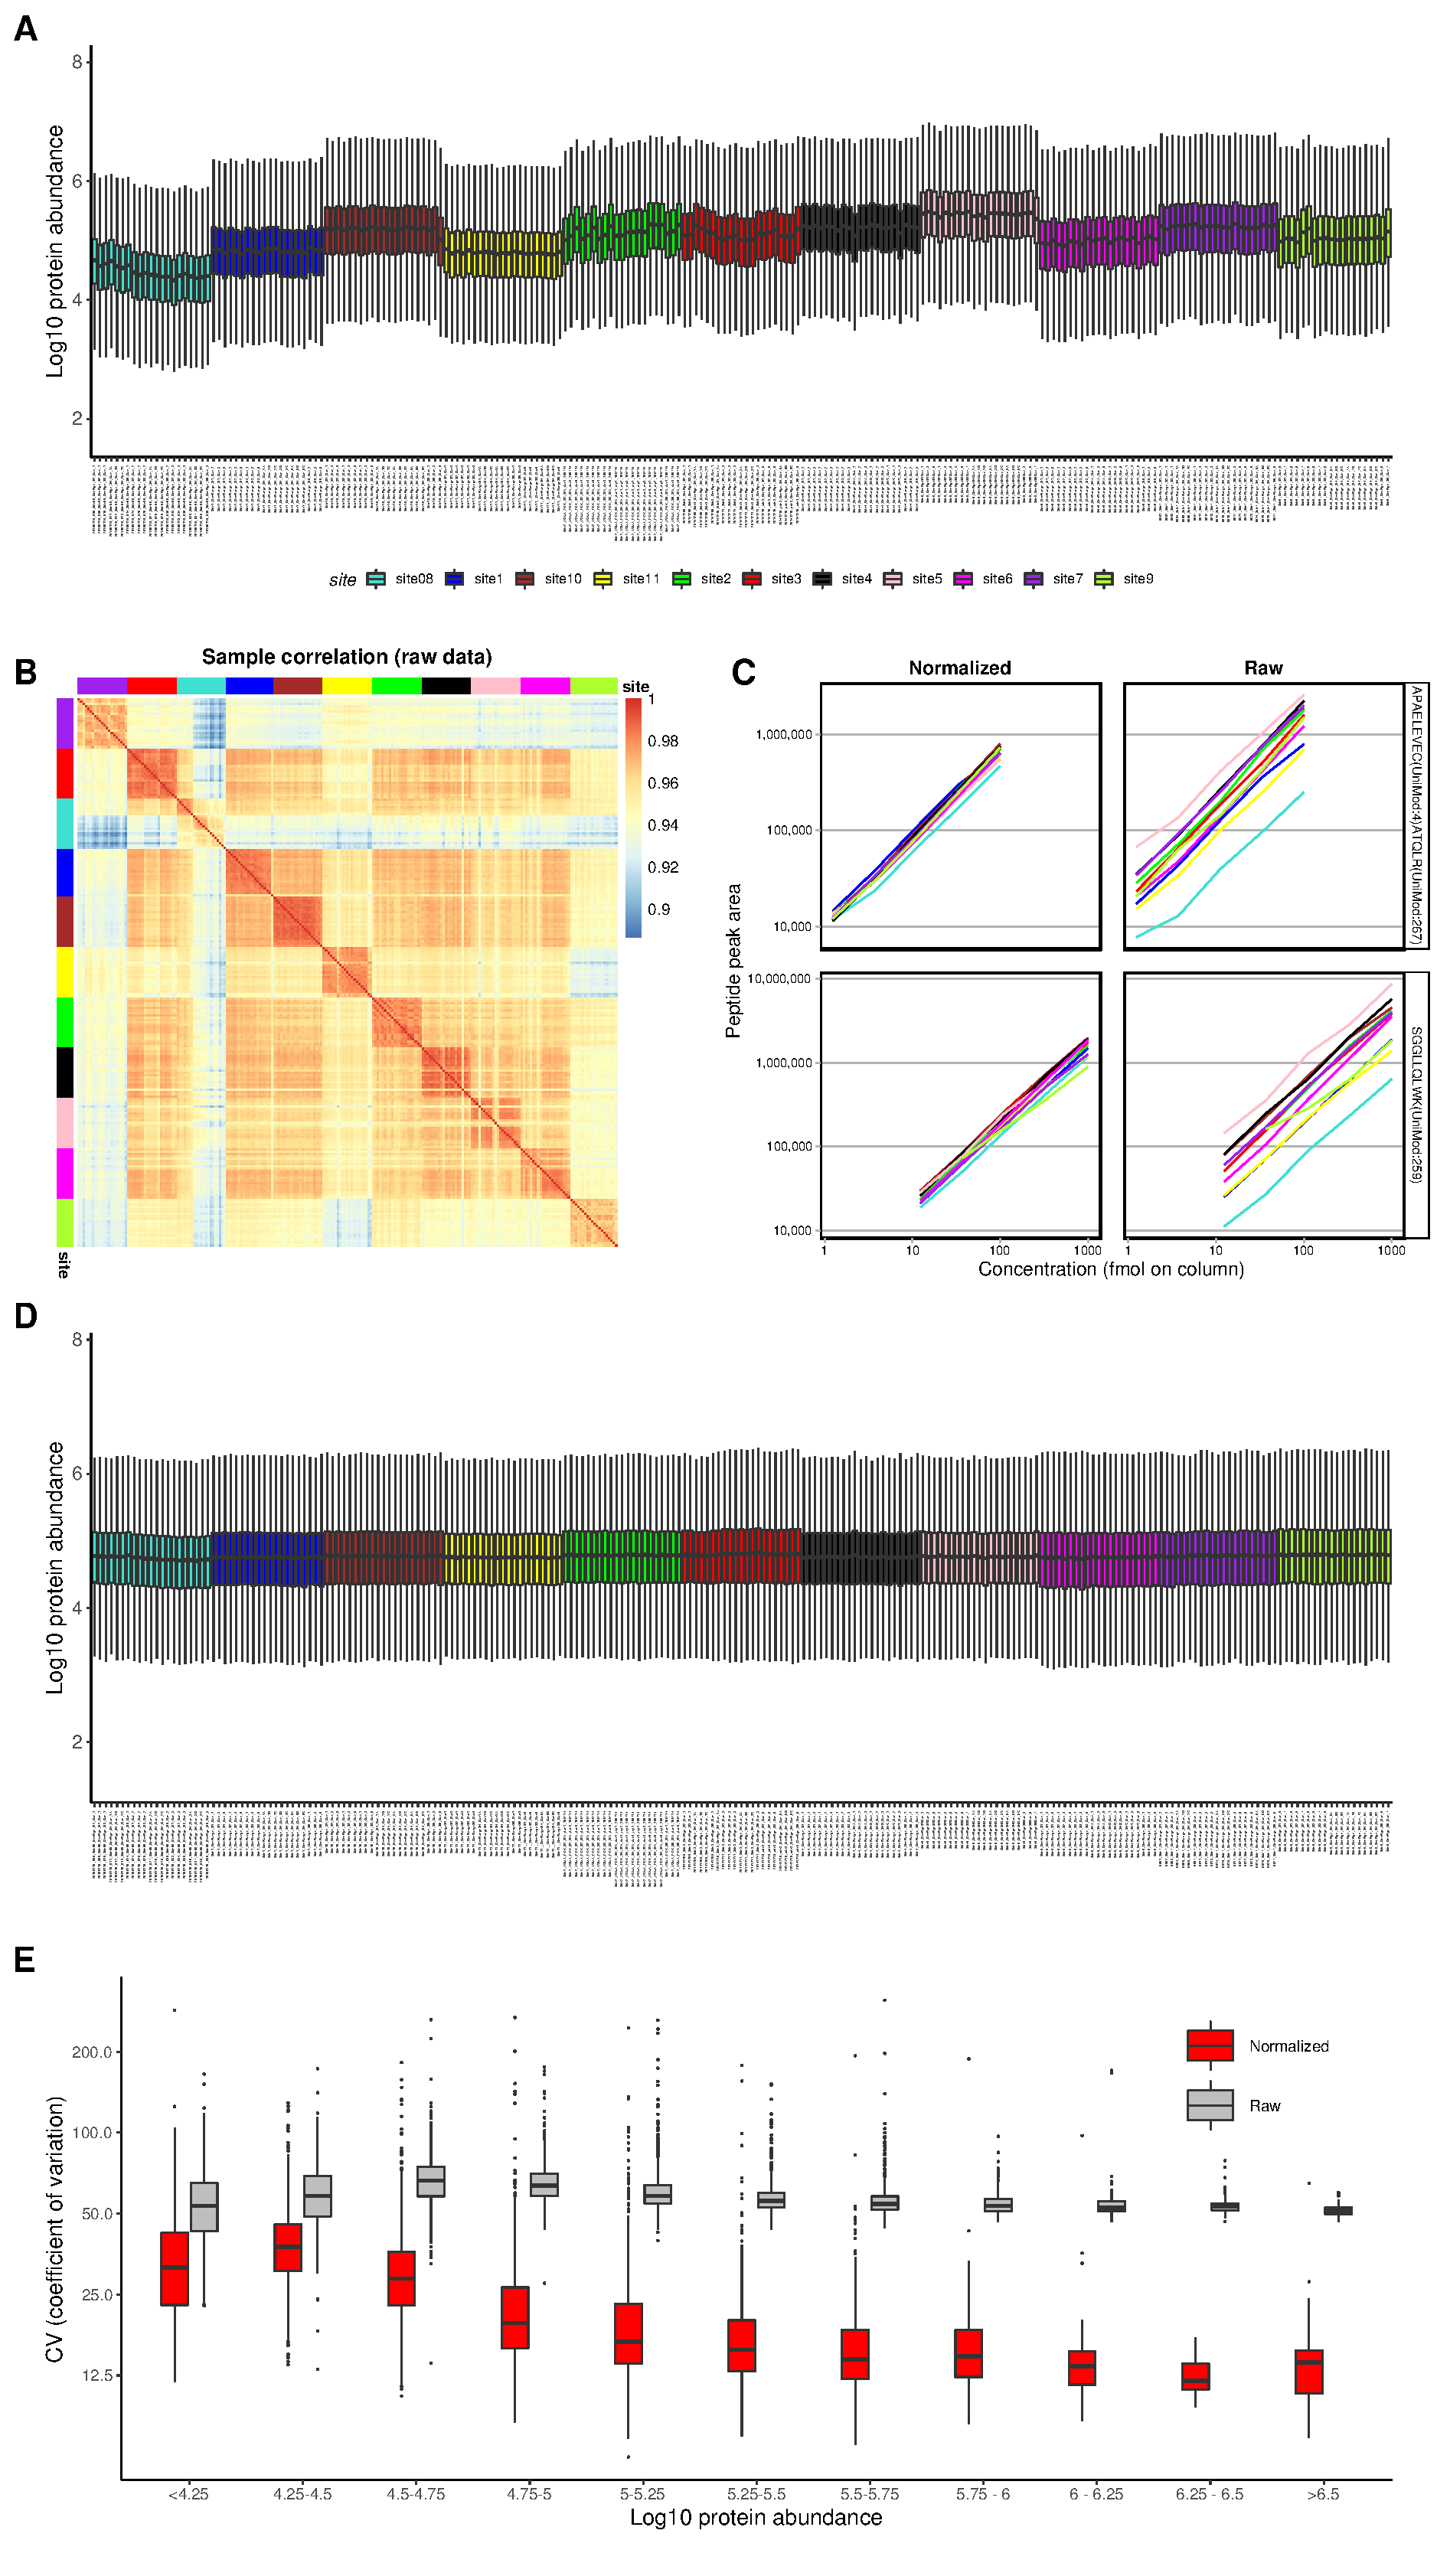
\includegraphics[width=\textwidth,height=.9\textheight,keepaspectratio]{figures/Supp_InterLab.pdf}
	\caption{\textbf{Batch effects in InterLab study}\\
		 \footnotesize  (A) Boxplots of raw sample intensities colored by MS spectra acquisition sites; (B) Sample correlation heatmap, top row and left column colored by MS spectra acquisition sites, used as a quality control; (C) Comparison of two spike-in peptide quantification in raw and normalized data; (D) Boxplots of median-normalized sample intensities; (E) Quality control by comparing coefficient of variance (CV) for proteins, binned by Log10 abundance.}
	\label{fig:batch_figS1_InterLab}
\end{figure}

\begin{figure}
	%\center
	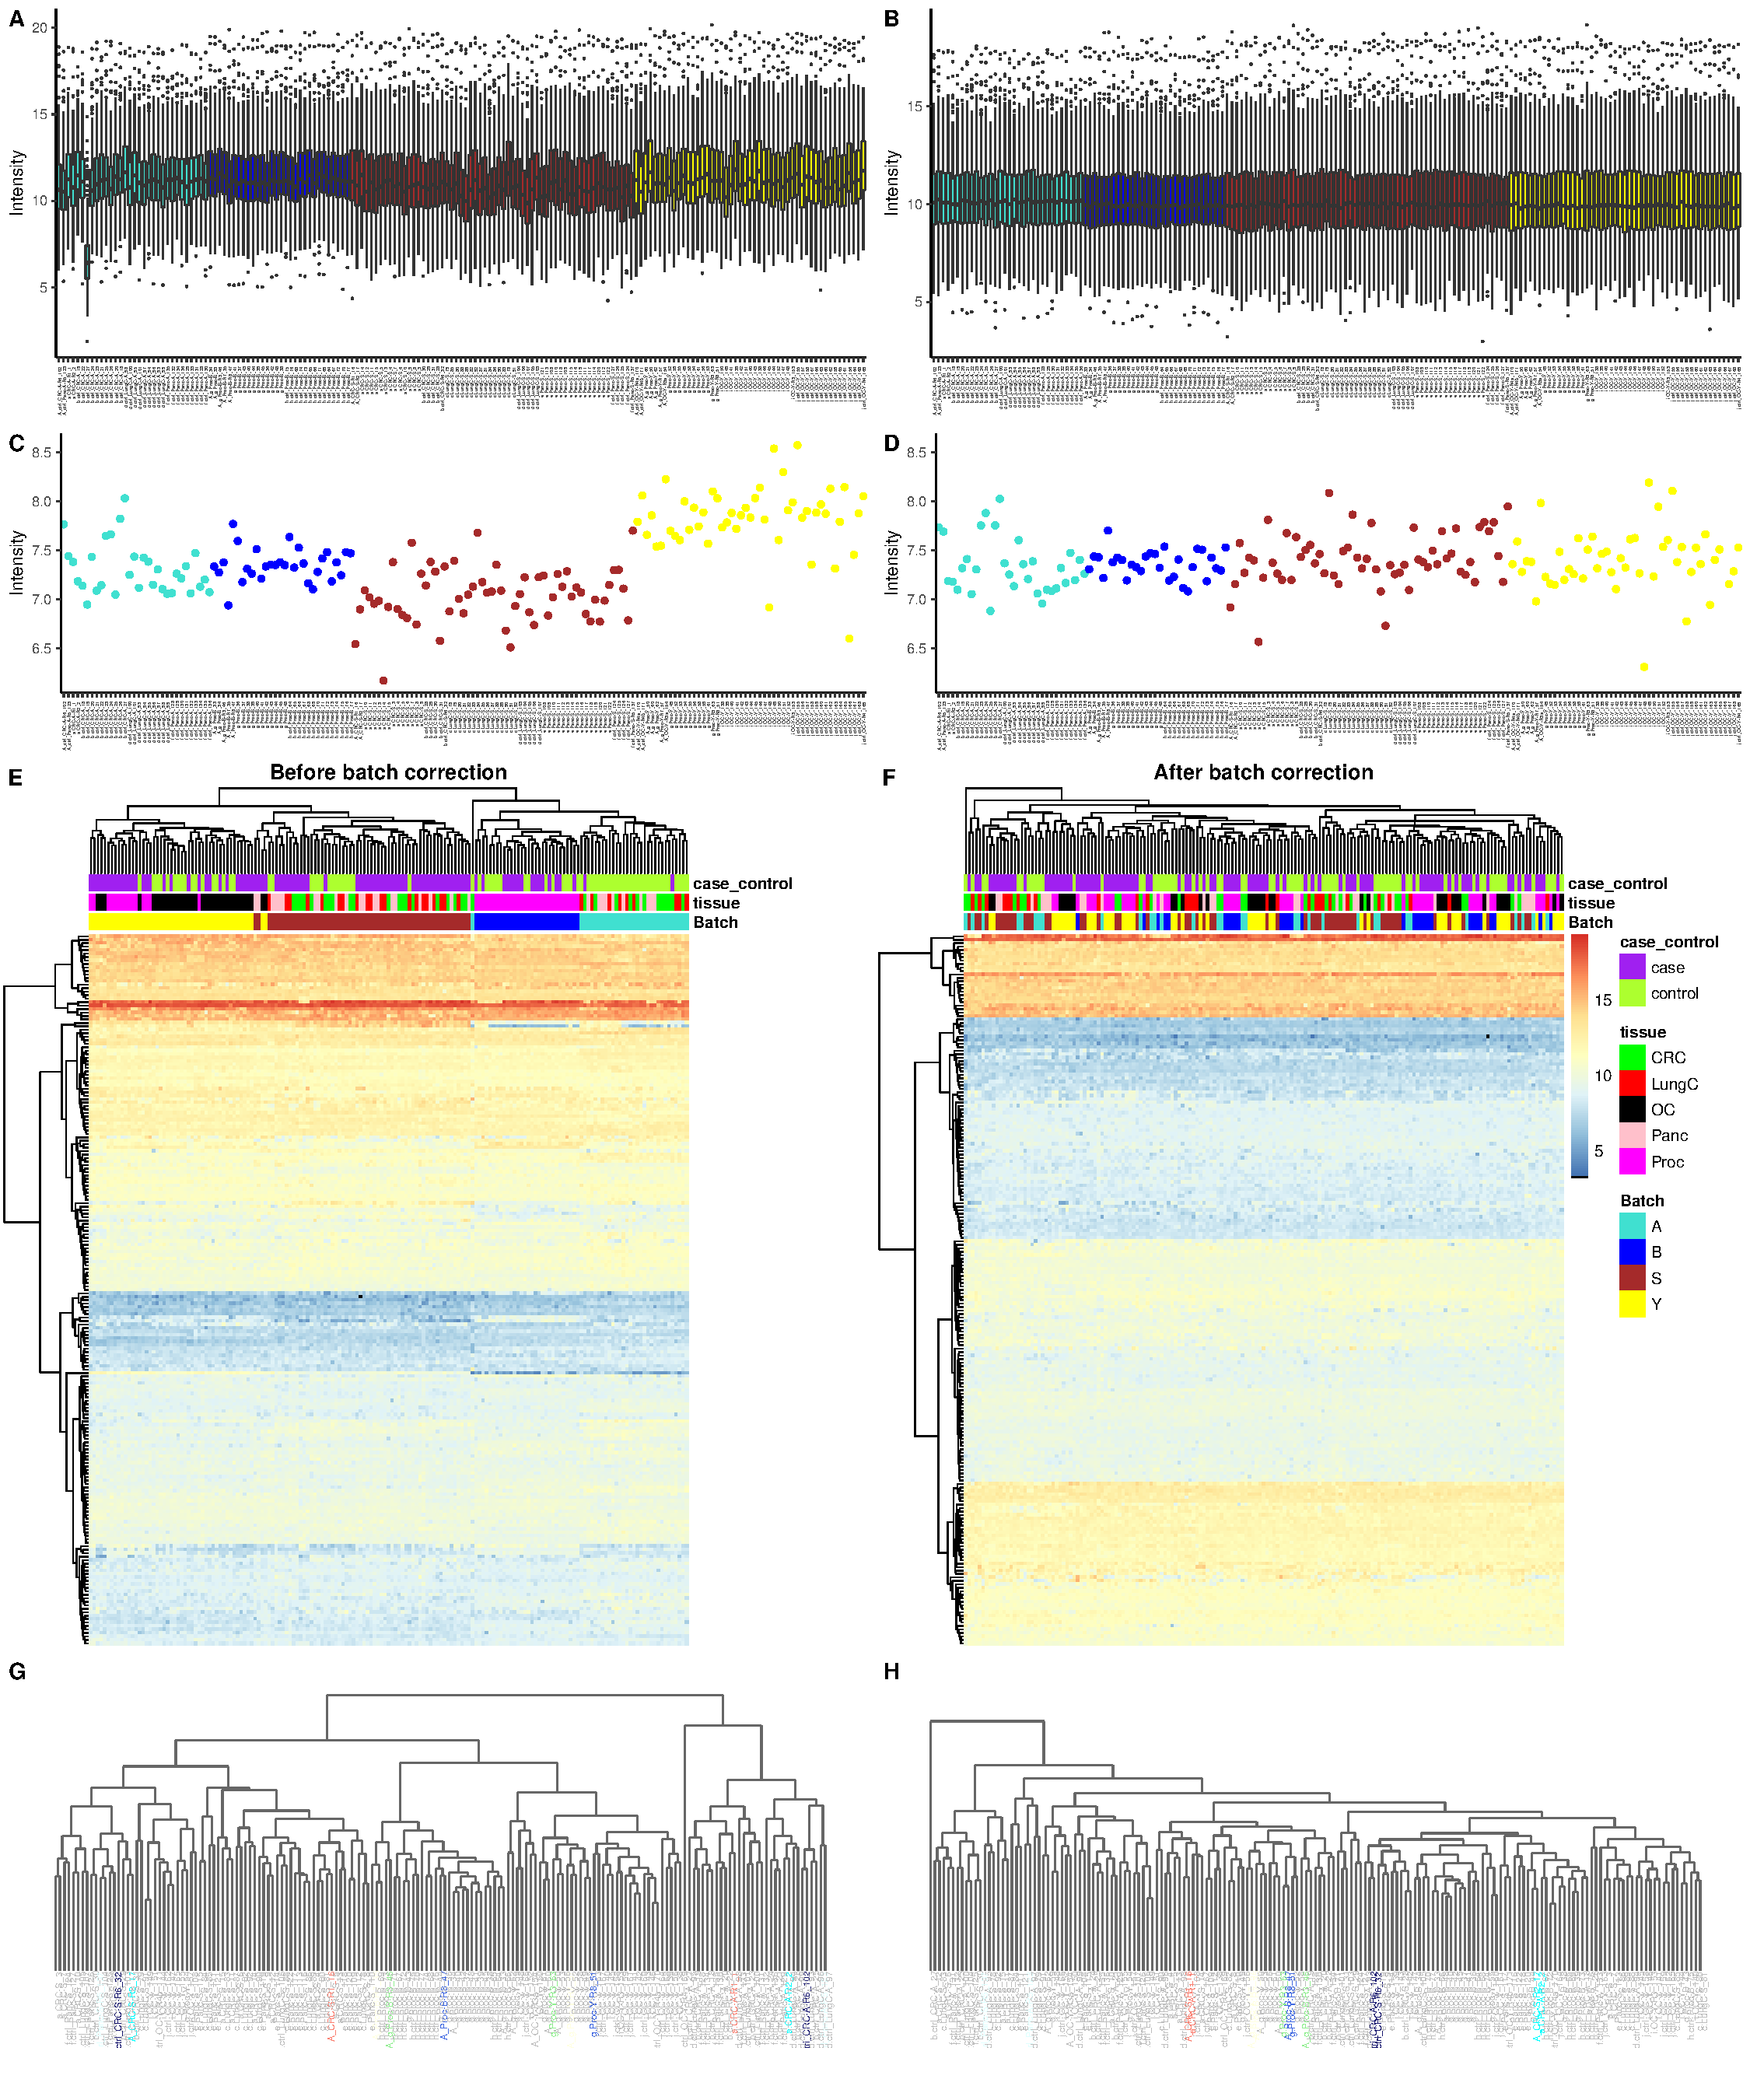
\includegraphics[width=\textwidth]{figures/Supp_Fig2_PanCancer}
	
	\caption{\textbf{Batch effects in PanCancer study} \\
		\footnotesize (A) Boxplots of raw sample intensities colored colored by digestion batch; (B) Boxplots of normalized sample intensities colored colored by digestion batch; 
		(C) Intensity of spike-in Fetubin in raw data; (D) Intensity of spike-in Fetubin in batch corrected data; (E) Hierarchical clustering and the heatmap of raw protein-level data; (F) Hierarchical clustering and the heatmap of batch corrected protein-level data; (G) Hierarchical clustering of normalized data with Manhattan distance, with replicated samples colored; (H) Hierarchical clustering of batch corrected data with Manhattan distance, with replicated samples colored.}
	\label{fig:batch_figS2_PanCancer}
\end{figure}


\end{document}
